% Exemplo de dissertação do INF-UFG com texto em portugues formatado com LaTeX
\documentclass[monografia, nocolorlinks]{inf-ufg}
% Opções da classe inf-ufg (ao usar mais de uma, separe por vírgulas)
%   [tese]         -> Tese de doutorado.
%   [dissertacao]  -> Dissertação de mestrado (padrão).
%   [monografia]   -> Monografia de especialização.
%   [relatorio]    -> Relatório final de graduação.
%   [abnt]         -> Usa o estilo "abnt-alf" de citação bibliográfica.
%   [nocolorlinks] -> Os links de navegação no texto ficam na cor preta.
%                     Use esta opção para gerar o arquivo para impressão
%                     da versão final do seu texto!!!

%----------------------------------------------------- INICIO DO DOCUMENTO %
\begin{document}

%------------------------------------------ AUTOR, TÍTULO E DATA DE DEFESA %
\autor{Josemar Pereira Rincon}
\autorR{Pereira Rincon, Josemar}

\titulo{\text Aplicação de visão computacional no teste palográfico \text}
%\subtitulo{\textless Subtítulo do Trabalho\textgreater}%

\cidade{Goiânia}
\dia{13}
\mes{09}
\ano{2019} % Formato numérico: \dia{01}, \mes{01} e \ano{2009}

%-------------------------------------------------------------- ORIENTADOR %
\orientador{ Dr. Eliomar Araújo de Lima}
\orientadorR{Araújo de Lima, Eliomar}
% Use os comandos a seguir se for Orientadora e nao Orientador.
%\orientadora{\textless Nome da Orientadora\textgreater}
%\orientadoraR{\textless Nome Reverso da Orientadora\textgreater}

%\coorientador{\textless Nome do Co-orientador\textgreater}
%\coorientadorR{\textless Nome Reverso do Co-orientador\textgreater}
% Use os comandos a seguir se for Co-orientadora e nao Coorientador.
%\coorientadora{\textless Nome da Co-orientadora\textgreater}
%\coorientadoraR{\textless Nome Reverso da Co-orientadora\textgreater}

%-------------------------------------------------- INSTITUIÇÃO E PROGRAMA %
\universidade{Universidade Federal de Goiás}
\uni{UFG}
\unidade{Insituto de Informática}
\departamento{} % Unidades com mais de um departamento.

%\universidadeco{\textless Nome da Universidade do Co-orientador\textgreater}
%\unico{\textless Sigla da Universidade do Co-orientador\textgreater}
%\unidadeco{\textless Nome da Unidade Acadêmica do Co-orientador\textgreater}

\programa{Design de Sistemas e Soluções de Business Intelligence}
\concentracao{Sistemas de Informação}

%-------------------------------------------------- ELEMENTOS PRÉ-TEXTUAIS %
\capa    % Gera o modelo da capa externa do trabalho
\publica % Gera a autorização para publicação em formato eletrônico
\rosto   % Primeira folha interna do trabalho

%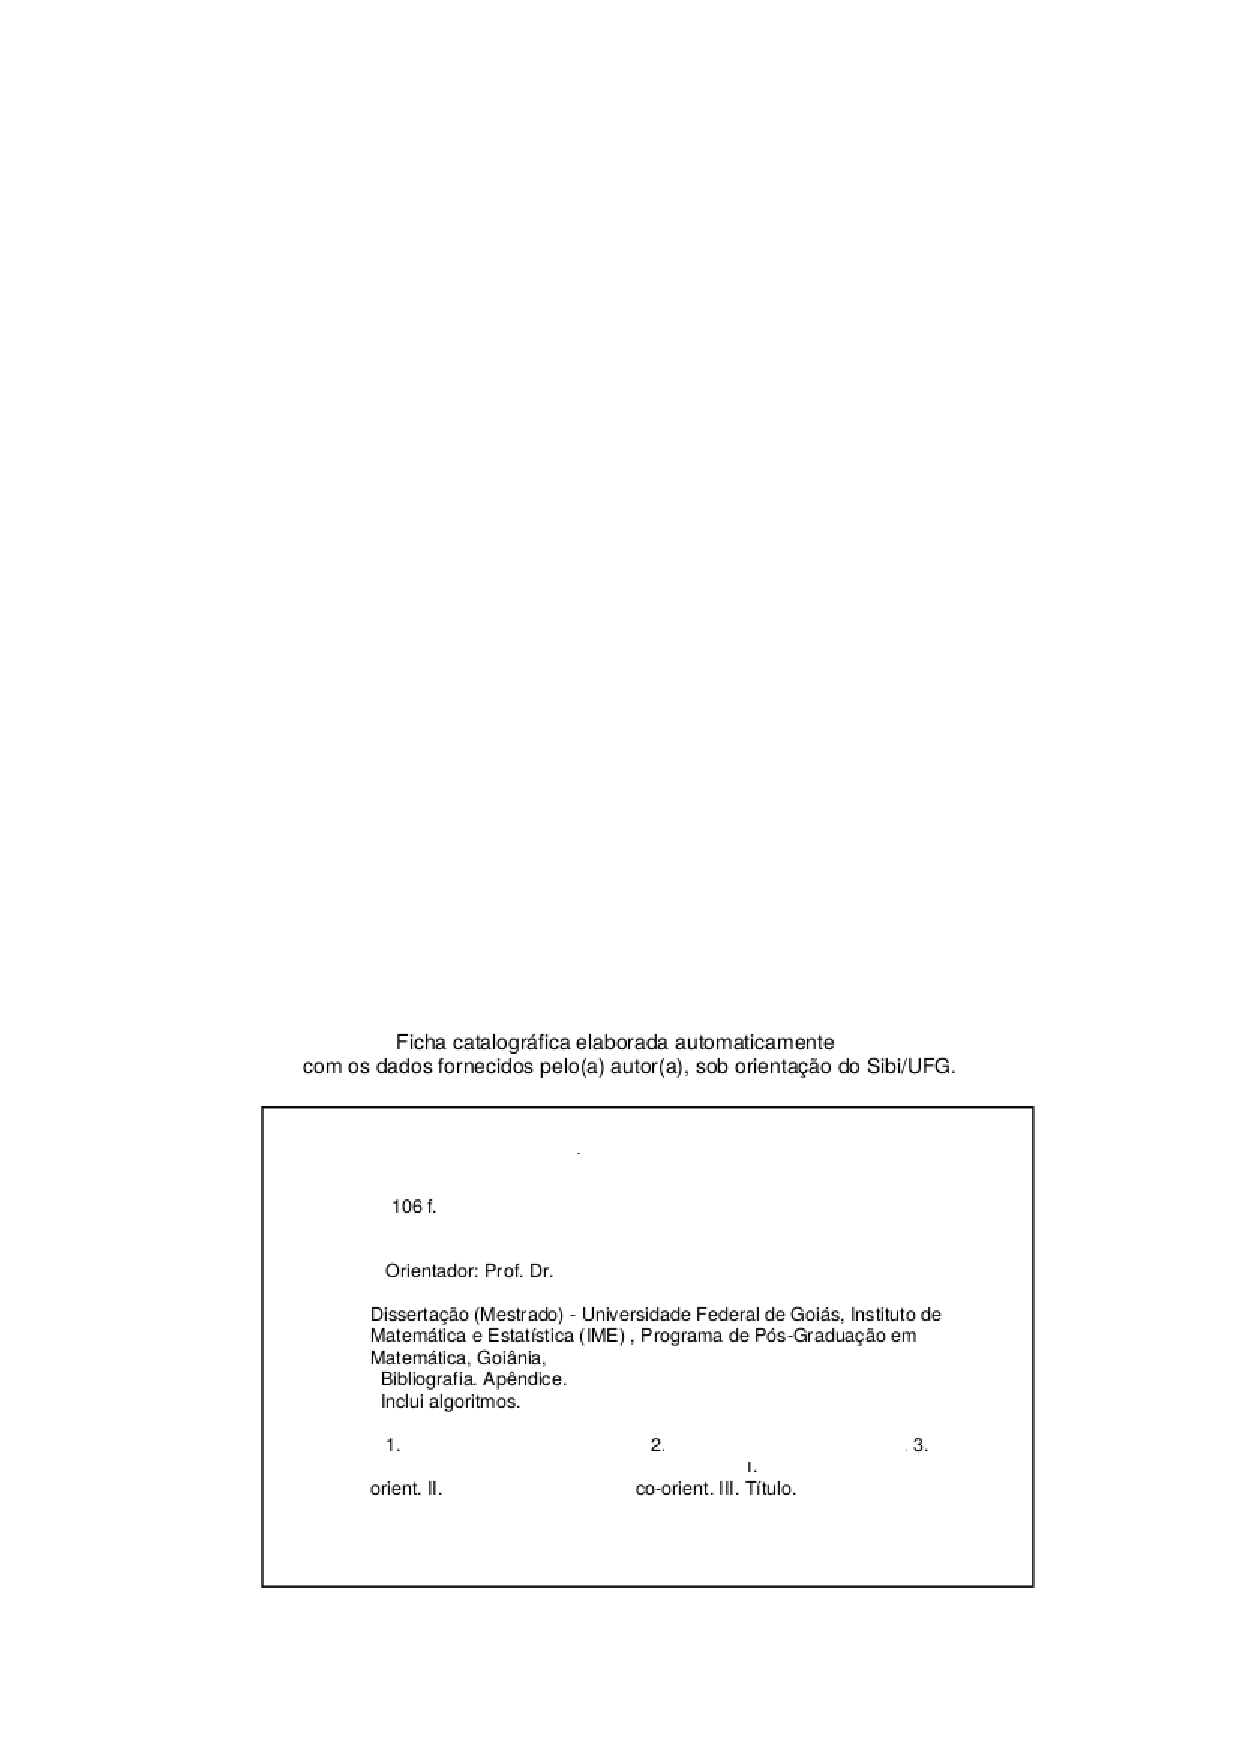
\includepdf[pages={1},templatesize={250mm}{297mm}]{./pre/FichaCatalografica.pdf}  %Ficha Catalográfica expedida pela secretaria do programa
\begin{aprovacao}
\banca{Dr. Vinícius Sebba Patto}{Instituto de Informática\ -- UFG}
\profa{ Dra. Nádia Félix Felipe da Silva}{Instituto de Informática\ -- UFG}
% Use o comando \profa se o membro da banca for do sexo feminino.
%\banca{Dr. Membro Externo}{Faculdade de Fora\ -- FF}
\end{aprovacao}
%\direitos{\textless Texto com um perfil resumido do autor do trabalho. Por exemplo: (Graduou--se em Artes Cênicas na UFG - Universidade Federal de Goiás. Durante sua graduação, foi monitor no departamento de Filosofia da UFG e pesquisador do CNPq em um trabalho de iniciação científica no departamento de Biologia. Durante o Mestrado, na USP - Universidade de São Paulo, foi bolsista da FAPESP e desenvolveu um trabalho teórico na resolução do Problema das Torres de Hanói. Atualmente desenvolve soluções para problemas de balanceamento de ração para a pecuária de corte.) \textgreater}


\begin{dedicatoria}
 Dedico esse trabalho a Deus que me da forças e saúde para ir além  e a minha querida esposa.
\end{dedicatoria}
\begin{agradecimentos}
  Agradeço a Deus por  me dar sabedoria para superar todos os desafios durante essa jornada. 

Ao meu orientador, Prof. Dr. Eliomar Araújo de Lima, pelo conhecimento transmitido, paciência e confiança.

Aos meus colegas de curso pelo aprendizado e conhecimentos compartilhados. 

À SESGO, por ter me proporcionado crescimento profissional e pessoal, especialmente ao Carlos Augusto Tibiriçá e a Luiselena Luna Esmeraldo que me ajudaram e me incentivaram.

Aos meus pais, Maria e Divino, pelo amor e por sempre investirem e acreditarem em mim.

À minha esposa, Juliete, pela paciência, compreensão, carinho e amor. 

Agradeço às pessoas que ajudaram direta ou indiretamente na
realização deste trabalho.

\end{agradecimentos}



\epigrafe{  " Uma imagem vale mais que mil palavras! " }
{Confúcio}
{}

\chaves{ teste psicológico, Opencv, processamento de imagens, celular. }

\begin{resumo} 
A análise do teste palográfico é feita tipicamente de forma manual pelo profissional de psicologia, exigindo a contagem de cada palo ou traço vertical, que uma pessoa consegue expressar em uma folha de papel. O teste pode ser aplicado individualmente ou em grupo, sendo o processo de contagem exaustivo, demorado e passível de erro humano. Com o objetivo de automatizar esse processo, uma solução foi proposta utilizando-se da técnica de visão computacional, baseada na biblioteca Opencv com linguagem, Python, possibilitando realizar o pré-processamento, segmentação, representação e reconhecimento, aplicadas nas imagens capturadas por smartphone em um ambiente com iluminação homogênea. Os resultados permitiram identificar cada traço e contá-los de maneira ordenada por intervalos de tempo, sugerindo um cenário promissor para a análise quantitativa do teste palográfico de maneira automática.
\end{resumo}


\keys{ psychological test, OpenCV, image processing, cell phone.}

\begin{abstract}{\textless Aplicação de visão computacional para contagem
dos palos no teste palográfico\textgreater}
Analysis of the palographic test is typically done manually by the psychologist, requiring the counting of each Palo or vertical line, that a person can express on a sheet of paper. The test can be applied individually or in groups, the counting process being exhaustive, time consuming and subject to human error. Aiming to automate this process, a solution was proposed using computer vision technique, based on Python Opencv library, enabling you to perform preprocessing, segmentation, representation and recognition, applied to images captured by smartphone in an environment with homogeneous lighting. The results allowed us to identify each trace and count them in an orderly manner by time intervals,, suggesting a promising scenario for the quantitative analysis of the palographic test automatically.

\end{abstract}



\tabelas[figtab]
%Opções:
%nada [] -> Gera apenas o sumário
%fig     -> Gera o sumário e a lista de figuras
%tab     -> Sumário e lista de tabelas
%alg     -> Sumário e lista de algoritmos
%cod     -> Sumário e lista de códigos de programas
%
% Pode-se usar qualquer combinação dessas opções.
% Por exemplo:
%  figtab       -> Sumário e listas de figuras e tabelas
%  figtabcod    -> Sumário e listas de figuras, tabelas e
%                  códigos de programas
%  figtabalg    -> Sumário e listas de figuras, tabelas e algoritmos
%  figtabalgcod -> Sumário e listas de figuras, tabelas, algoritmos e
%                  códigos de programas



%--------------------------------------------------------------- CAPÍTULOS %
\chapter{Introdução}
\label{cap:intro}


O desenvolvimento tecnológico tem avançado muito nos últimos tempos, principalmente na computação móvel por exemplo os nossos celulares  estão com um poder de processamento cada vez maior e o acesso a internet tem se popularizado cada vez mais, possibilitando o surgimentos de serviços inovadores como aberturas de contas bancárias, fazer pagamentos utilizando a câmera como leitor de código de barras, pedir um carro para levá-lo onde quiser, escanear documentos usando a câmera do celular, pedir comida, reservar um lugar para passar uns dias, dentre outros. Nesse sentido, vemos que muitos setores de diversas áreas buscam  adaptar seus produtos e serviços às exigências da atualidade.

A psicologia não está fora dessa evolução tecnológica, o que permite melhorar suas técnicas de investigação e as práticas que direcionam seus profissionais. O emprego da tecnologia contribui muito para os avanços que a área precisa, ao possibilitar, por exemplo, suporte ao profissional na execução das tarefas mecânicas, como a de contagem, correção e conversão de pontuações nas ocasiões em que os testes são utilizados \cite{psico-artigo}

Com o uso de recursos tecnológicos o psicologo aperfeiçoa sua prática, uma vez que, além de economizar tempo, reduzem erros de medições nos testes psicológicos, fazendo com que as avaliações sejam mais precisas e confiáveis.

Apesar dos avanços da informática na área da psicologia, poucos serviços ou produtos voltados aos testes psicológicos foram desenvolvidos para  dispositivos móveis.

\section{Motivação}
\label{sec:motiv}
Apesar de alguns avanços conseguidos com o uso da informática na psicologia alguns processos ainda são realizados de maneira manual, como a contagem dos palos no teste palográfico.
O teste palográfico pode ser aplicado em grupo ou individual, cada indivíduo pode fazer mais de 1000 palos em uma folha de papel durante o teste, o aplicador ao fazer a correção tem que contar manualmente cada palo para fazer sua avaliação quantitativa, isso é bastante exaustivo e demorado para o profissional principalmente se tiver que fazer varias correções em um único dia, por exemplo no Detran quantas pessoas fazem esse teste por dia? analisando os dados no portal do Detran \footnote{http://inside.detran.go.gov.br/habilitacao/index.htm} vemos que houve uma variação na quantidade de condutores de 3599 entre os meses de julho e agosto de 2019,  isso significa que nesse período foram realizados por dia uma média de 116 testes palográficos, e isso não é tudo, pois o psicólogo ao fazer a correção do teste  precisa realizar também a análise qualitativa, que envolve outros aspectos dos palos. 

Outro problema resultante da contagem manual é que devido esse processo ser exaustivo, pois os aplicadores precisam contar os palos de muitos testes realizados em certo período, isso pode gerar erros na contagem. O desenvolvimento de uma forma eficaz e prática de  contagem dos palos agilizaria muito o trabalho dos aplicadores do teste palográfico, aumentando sua produtividade e qualidade de vida. O que traria um grande benefício para os profissionais dessa área como um todo.


\section{Objetivos}
\label{sec:motiv}

O objetivo geral deste trabalho é propor a utilização de técnicas de  visão computacional e processamento de imagens para  aprimorar e auxiliar o processo de avaliação quantitativa do teste palográfico. Espera-se neste trabalho que o algoritmo desenvolvido possa realizar a identificação e contagem ordenada dos palos em imagens obtidas por meio de um celular. Para ficar claro esse trabalho não tem o objetivo de desenvolver o aplicativo para o celular, apenas o algoritmo que visa extrair as informações da imagem podendo  ser disponibilizadas como API REST em futuras aplicações. Para alcançar esse objetivo, pretende-se realizar os seguintes objetivos específicos:
\begin{itemize}
\item Realizar um estudo sobre a aplicação do teste palográfico;
\item Identificar potenciais técnicas de processamento de imagens pra localização dos palos;
\item fazer experimentos com algoritmos que possam extrair características relevantes para a identificação dos palos;
\item Elaborar um algoritmo de contagem dos objetos localizados, os palos;
\item Avaliação dos resultados obtidos.
\end{itemize}

Dessa maneira, seria possível que o  resultante deste trabalho produza um protótipo capaz de realizar a contagem automática dos palos, sem a necessidade de uso de um hardware específico como ocorre em \cite{skip2018}, apenas com o uso de imagem feito por celular ? É o que este estudo pretende responder.



\section{Trabalhos relacionados}
\label{sec:tbrel}

Nesta seção são apresentados alguns trabalhos relacionados que foram encontrados na literatura. Mostrando aos leitores que a área citada neste trabalho trata-se de fontes de interesse de estudos científicos.

Diversos trabalhos de processamentos de imagens e visão computacional com foco em detecção e contagem de objetos são encontrados na literatura. No trabalho apresentado em \cite{SANTOS2013}  o objetivo é a contagem automática de veículos em vias. Neste trabalho foi aplicado técnica de segmentação estatística, baseada em regressão linear não paramétrica na parte de segmentação do contador. O trabalho foi dividido em três módulos, uma para a segmentação, outro para rastreamento e outro para o reconhecimento. As técnicas utilizadas nos módulos foram segmentação por subtração do fundo, filtros kalman no rastreamento e rede neural perceptron multicamadas, treinada por retropropagação no reconhecimento. Os resultados foram satisfatórios, capaz de fazer a contagem de três classes de veículos, carro, caminhão, e ônibus com taxa de acerto em torno de 70\% no melhor caso e 50\% no pior. Esse projeto foi desenvolvido na linguagem C e C++/CLI, foi utilizada também no processamento de imagens a biblioteca OpenCV.

É apresentado em \cite{SILVA2012} um trabalho sobre contagem semi-automática e automática dos ovos do mosquito da dengue como uso de processamento de imagens adquiridas de palhetas das ovitrampas , armadilhas especiais para deposição e contagem dos ovos do mosquito. O sistema desenvolvido é baseado em uma plataforma óptica, uma interface homem-máquina e um software de aquisição de imagem. A contagem semi-automática gerou um ganho de velocidade na contagem  de três vezes com relação a contagem manual. A contagem automática dos ovos baseia-se nos processo de segmentação (realizada por cor e por limiarização, filtragem(espacial e morfológica) e quantificação. Foram utilizadas 100 imagens obtendo um erro global de 2.67\%. Obtendo resultados satisfatórios.

Outro trabalho semelhante, é apresentado em \cite{BANKE2012} que descreve o desenvolvimento de um sistema para contagem automática de células sanguíneas em campos microscópicos por meio de visão computacional. No pré-processamento das imagens foram utilizadas técnicas para redução de ruídos como filtros da mediana, algorítimos de inundação que combina as técnicas de detecção de bordas, limiarização e crescimento de região, na segmentação, operações morfológicas de erosão e dilatação, na etapa de descrição foi utilizado algoritmos de rotulação de componentes conexos, no qual é gerado uma lista que contém a posição de cada elemento, em seguida, é feito o cálculo da área com base no número de pontos pertencentes ao mesmo. Na identificação é feito a contagem verificando-se a área de cada elemento com base em um valor aceitável e descartando os que estiverem fora desse valor. 
Sistema implementado em C++, com uso da biblioteca OpenCV.

O trabalho proposto em \cite{SILVA2018} tem como objetivo utilizar técnicas de aprendizado de máquina e visão computacional para detecção e contagem de árvores em uma plantação de eucaliptos. Foram utilizados modelos de redes neurais convolucionais existentes na plataforma TensorFlow. As imagens para treinamento da rede foram obtidas por um VANT(Veículos Aéreos Não Tripulados) através de um sobrevoo na plantação. Dos modelos testados o que se saiu melhor foi o Faster R-CNN(\textit{Region-proposal Convolutional Neural Network}) Resnet 101 com precisão de 95\% contando 7471 das 7866 plantas de eucaliptos, com apenas 395 resultados falsos 5\%.  Foi utilizado no desenvolvimento a linguagem Python e a biblioteca de aprendizado de maquina TensorFlow da Google.

O único projeto relacionado com a contagem dos palos encontrado foi um software chamado SKIP \cite{skip-artigo}, que faz a análise quantitativa e qualitativa dos palos, através de imagens capturadas por scanners específicos instalados em um computador. A vantagem do protótipo desenvolvido neste trabalho com relação ao software SKIP e que não é preciso adquirir nenhum hardware específico para utilizá-lo, e a desvantagem é que o protótipo ainda não faz a análise qualitativa, que ficará para trabalhos futuros.




\section{Organização do texto}
\label{sec:motiv}

O próximo Capítulo traz a fundamentação teórica, detalhando e reunindo os conceitos científicos sobre o teste palográfico, processamento Digital de Imagens e visão computacional. No Capítulo 3, é mostrado todo o processo de desenvolvimento do algorítimo e técnicas utilizadas neste trabalho. No Capítulo 4, é apresentado toda a análise referente à execução de testes e resultados alcançados no protótipo. No Capítulo 5, temos a conclusão do trabalho proposto e abordagem de trabalhos futuros.

\chapter{Revisão da Literatura}
\label{cap:descr}

%% - - - - - - - - - - - - - - - - - - - - - - - - - - - - - - - - - - -
\section{O Teste palográfico}
\label{sec:testep}
O teste dos palos tem como objetivo fazer uma avaliação da personalidade do indivíduo. É muito utilizado em empresas no recrutamento e seleção, para conseguir selecionar os melhores profissionais do mercado e garantir compatibilidade entre os profissionais selecionados com as exigências da vaga. 

O teste palográfico foi desenvolvido na Espanha e trazido para o Brasil por Agostinho Minicucci na década de 1970. O instrumento é considerado um teste expressivo de personalidade,  que tem como base teórica, questões relativas ao comportamento expressivo e técnicas gráficas para avaliação da personalidade.\cite{ibapnet2012} Personalidade é o conjunto de características  físicas, genéticas e sociais que faz de um individuo diferente e único. \cite{dicio2018}

O teste palográfico depende da forma como a pessoa traça riscos numa folha, o psicólogo irá fazer uma análise da sua personalidade, verificando dados de ritmo e qualidade de trabalho, fatigabilidade, inibição, elação, depressão, temperamento, inteligencia, etc. \cite{manualPsico2010}

\section{Aplicação e correção do Teste}
\label{sec:formateste}
Ao aplicar o teste o psicologo não se diz aos candidatos do que se trata, apenas diz que é um teste de resistência e velocidade.

É fornecida uma folha em branco sem linhas. Nessa folha vem de exemplo 3 palos no começo da folha e abaixo desses 3 palos tem mais 1 palo impresso, com altura de 7mm,  e espaçados de 2 em 2 mm que devem ser replicados por quem for fazer o teste. A pessoa deve fazer de lápis, riscos verticais o quanto puder e o mais perfeito possível, no tempo de 5 minutos. \cite{manualPsico2010}

Para cada minuto o psicologo dará o comando "sinal", então a pessoa deverá riscar um traço na horizontal, e continuar a fazer os traços na vertical. ex:
|||||||||||||||||||-|||||||||||||||||-|||||||||||||||||||-|||||||||||||||||||-|||||||||||||||||
Antes de começar há um treino inicial e só depois é iniciando o teste. \cite{manualPsico2010}

O teste é muito utilizado em RH para fazer contratações  e no Detran (para autorizar a carteira de habilitação). \cite{kenoby2017}

A avaliação do teste palográfico é abordada de maneira quantitativa e qualitativa\footnote{ Para mais informações sobre a parte qualitativa acesse o manual do psicotécnico p. 355: https://aderivaldo23.files.wordpress.com/2008/06/37527582-manual-do-psicotecnico-1.pdf.}, esse trabalho se restringe apenas a parte quantitativa.

\subsection{Folhas do teste}
\label{sec:folhasTeste}

Existem dois modelos de folhas para realização do teste, um grande (36,3 x27,4 cm) e outro reduzido (21,5 x 32,0 cm). Em geral o mais utilizado é o reduzido, devido a limitação do tamanho das carteiras dos examinadores. Neste trabalho os testes focaram no modelo reduzido.\cite{passetestepalografico2013}


\begin{figure}[H]
 \centering
 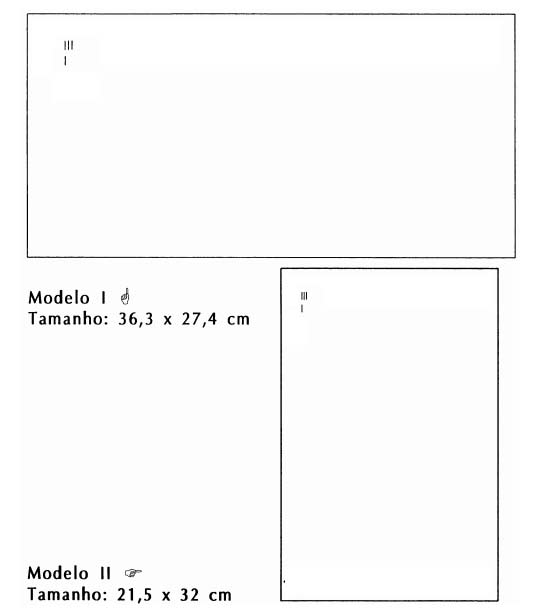
\includegraphics[width=0.76\textwidth]{./fig/palos/folhas}
 \caption{Modelos de folhas para aplicação do teste palográfico.}
  Fonte: \cite{passetestepalografico2013}.
 \label{fig:folhas}
\end{figure}


\subsection{Avaliação Quantitativa}
\label{sub:avaquali}

Nessa análise são considerados produtividade, rítmo, e rendimento.

\subsubsection{Produtividade}
\label{subsub:avaquali}

É a quantidade total de riscos, somando-se os 5 tempos.
Segundo \cite{marcosjaime2013}  a produtividade pode ser analisada de acordo com a quantidade de palos que a pessoa conseguiu fazer, compara-se com uma faixa de valores padrão de acordo com sua escolaridade, para fazer a classificação conforme pode se ver abaixo.

Candidatos (as) com escolaridade NÍVEL MÉDIO
\begin{itemize}
\item Menor ou igual 313: Inferior ou Lento - Indica uma produtividade muito abaixo da média.
\item De 314 a 423: Média Inferior ou Baixa - Índice demonstra um rendimento no trabalho abaixo da média.
\item De 424 a 693: Média - Indica possuir produtividade mediana no trabalho.
\item De 694 a 936: Média Superior ou Alta - Denota possuir produtividade acima da média.
\item  A partir de 937: Superior ou Muito Alta - Este índice revela produtividade acentuada no trabalho, indicando rendimento bastante acima da média.
\end{itemize}

Candidatos com escolaridade até NÍVEL SUPERIOR :

\begin{itemize}
\item Até 396: Inferior ou Lento - Indica uma produtividade muito abaixo da média.
\item De 397 a 546: Média Inferior ou Baixa - Este índice denota um rendimento no trabalho abaixo da média.
\item De 547 a 830: Média - Indica possuir produtividade mediana no trabalho.
\item De 831 a 1059: Média Superior ou Alta - Denota possuir produtividade acima da média.
\item A partir de 1060: Superior ou Muito Alta - Este índice revela produtividade acentuada no
trabalho, indicando rendimento bastante acima da média.
\end{itemize}

\subsubsection{Ritmo}
\label{subsub:ritmo}

Na avaliação do ritmo faz-se a soma da diferença na quantidade de palos entre cada um dos 5 tempos, proporcional ao total de palos na soma dos 5 tempos. Quanto mais baixo o nível de oscilação do ritmo, melhor. Isso pode também ser chamado de NOR - (Nível de Oscilação Rítmica. A fórmula é: NOR= (soma das diferenças)*100/(total de palos).\cite{marcosjaime2013} 

Ex: Palos 107/103/115/110/109 = 544 (total de palos)
Diferença: 4/12/5/1 = 22 (soma das diferenças)
(22x100)/544 = 4 (NOR)

De acordo com a o seu valor de NOR o avaliado pode ser classificado utilizando-se a faixa de valores para o NOR conforme abaixo. \cite{marcosjaime2013}

\begin{itemize}
\item NOR: 0,0 a 2,1: Muito Baixo - Indica rígida regularidade na execução das tarefas, capaz de manter uma produtividade constante.
\item NOR: 2,2 a 4,0: Baixo - Revela produtividade estável no trabalho, capaz de manter rendimento constante.
\item NOR: 4,1 a 8,7: Médio - Revela alguma instabilidade em sua produtividade, porém sendo capaz de executar satisfatoriamente tarefas repetitivas.
\item NOR: 8,8 a 13,2: Alto - Indicativo de oscilações na produtividade e rendimento irregular no trabalho.
\item NOR: a partir de 13,3: Muito Alto – Revela preocupante oscilação na produtividade demonstrando rendimento bastante irregular.
\end{itemize}

\subsubsection{Rendimento}
\label{subsub:rend}

A análise do rendimento é feita por um gráfico que da uma visão mais clara da relação entre a produtividade e o ritmo. Aqui é analisado a qualidade do rendimento no trabalho e a tendência à exaustão. No gráfico é analisado os tempos x quantidade de palos sendo os tempos no eixo das abcissas e a quantidade de palos no eixo das ordenadas. Para que a oscilação na produtividade seja melhor observada, deve-se sempre fazer o eixo vertical partindo do zero \cite{psicohood2018}.

Abaixo mostro como é feito a analise do gráfico de rendimento com alguns exemplos segundo os autores \cite{psicohood2018} e \cite{manualPsico2010}.

\textbf{Equilibrado} (NOR entre 4 e 6, com produção média): indica capacidade e distribuição do tônus muscular de forma organizada e sistemática. Revela realização de trabalho uniforme.

Ex.:

\begin{table*}[hp]
\caption{Rendimento equilibrado \cite{psicohood2018} }
\label{tab:equilibrado}

\centering
\begin{tabular}{|l|c|c|c|c|c|c|}
\hline   \multicolumn{1}{|l|}{Tempos}   & 1     & 2     & 3    &  4     & 5     & Total \\ 
\hline Nº de traços & 120 & 130 & 125 & 133 & 142 & 650 \\ 
\hline    \multicolumn{2}{|l|}{ Diferenças}& 10   & 5     & 8     & 9     & 32\\ 
\hline NOR = 4,9\\
\cline{1-11}
\end{tabular} 

\end{table*}

\begin{figure}[H]
 \centering
 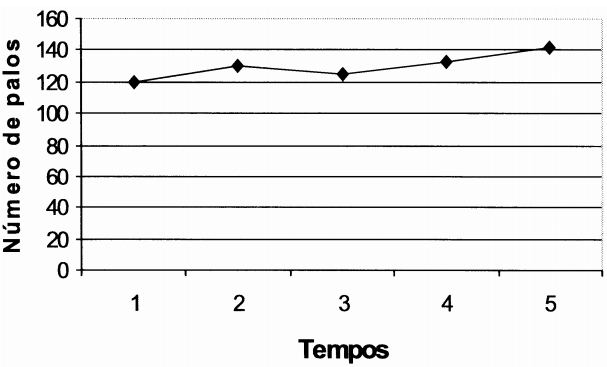
\includegraphics[width=0.76\textwidth]{./fig/grafico-rendimento/equilibrado}
 \caption{Rendimento equilibrado.}
  Fonte: \cite{psicohood2018}.
 \label{fig:folhas}
\end{figure}

\textbf{Rígido} (NOR entre 0 e 3, com produção média ou baixa): reflete pessoa obsessiva por detalhes e organização,
com rigidez da personalidade.

Ex.:
\begin{table*}[hp]
\caption{Rendimento rígido \cite{psicohood2018} }
\label{tab:rigido} 
\centering
\begin{tabular}{|l|c|c|c|c|c|c|}
\hline Tempos       & 1     & 2     & 3    &  4     & 5     & Total \\ 
\hline Nº de traços & 100 & 102 & 103 & 101 & 104 & 510 \\ 
\hline    \multicolumn{2}{|l|}{ Diferenças}& 2   & 1     & 2     & 3     & 8\\ 
\hline NOR = 1,6 \\ \cline{1-1}
\end{tabular} 

\end{table*}

\begin{figure}[H]
 \centering
 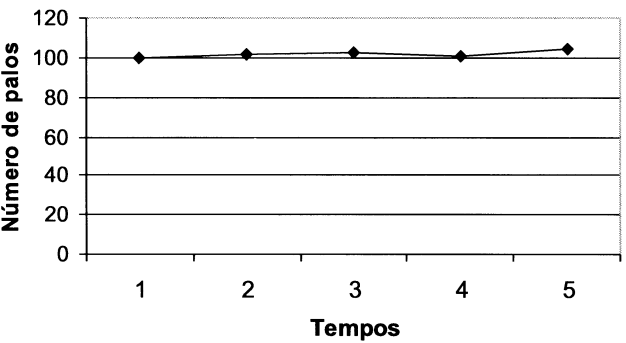
\includegraphics[width=0.76\textwidth]{./fig/grafico-rendimento/rigido}
 \caption{Rendimento rígido.}
  Fonte: \cite{psicohood2018}.
 \label{fig:folhas}
\end{figure}

\textbf{Ascendente ou crescente} (NOR acima de 6, com produção média): indica prudência diante de uma nova tarefa, mas aumenta a produção à medida que o indivíduo se sente mais seguro na situação. Também significa dinamismo e iniciativa.

Ex.:
\begin{table*}[hp]
\caption{Rendimento ascendente ou crescente \cite{psicohood2018} }
\label{tab:ascende} 
\centering
\begin{tabular}{|l|c|c|c|c|c|c|}
\hline Tempos       & 1     & 2     & 3    &  4     & 5     & Total \\ 
\hline Nº de traços & 110 & 125 & 135 & 140 & 155 & 665 \\ 
\hline    \multicolumn{2}{|l|}{ Diferenças}& 15   & 10     & 5     & 15    & 45\\ 
\hline NOR = 6,7\\  \cline{1-1}
\end{tabular} 

\end{table*}

\begin{figure}[H]
 \centering
 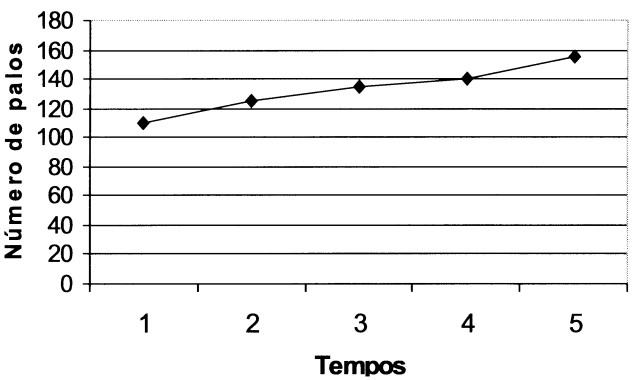
\includegraphics[width=0.76\textwidth]{./fig/grafico-rendimento/crescente}
 \caption{Rendimento ascendente ou crescente.}
  Fonte: \cite{psicohood2018}.
 \label{fig:ascende}
\end{figure}

\textbf{Descendente ou decrescente} (NOR acima de 6): é indicativo de cansaço, fadiga ou estresse, dificuldade de manter o tônus muscular, falta de ânimo e disposição. Pode refletir também tendência à depressão.

Ex.:

\begin{table*}[h]
\centering
\caption{Rendimento descendente ou decrescente \cite{psicohood2018} }

\label{tab:decrescente}


\begin{tabular}{|l|c|c|c|c|c|c|}
\hline Tempos       & 1     & 2     & 3    &  4     & 5     & Total \\ 
\hline Nº de traços & 180 & 175 & 150 & 143 & 125 & 773 \\ 
\hline    \multicolumn{2}{|l|}{ Diferenças}& 5   & 25    & 7     & 18    & 55\\ 
\hline NOR = 7,1\\
\cline{1-11}
\end{tabular} 

\end{table*}

\begin{figure}[H]
 \centering
 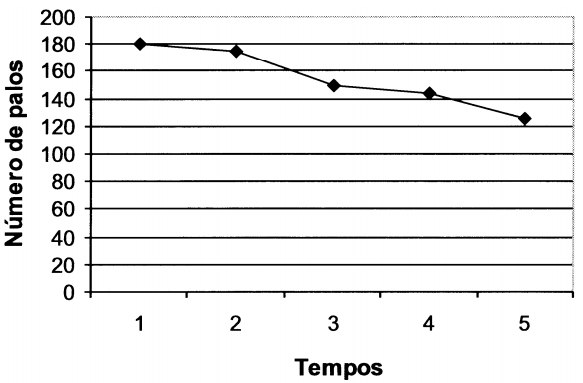
\includegraphics[width=0.76\textwidth]{./fig/grafico-rendimento/decrescente}
 \caption{Rendimento descendente ou decrescente.}
  Fonte: \cite{psicohood2018}.
 \label{fig:ascende}
\end{figure}


\textbf{Convexo ou parabólico} (NOR acima de 6): há um aumento da produção no 2º tempo, mantendo-se ou aumentando no 3º tempo, mas não continua com a disposição até o final da tarefa, voltando aproximadamente ao nível de produção inicial. Expressa ímpeto para iniciar as tarefas, que não se mantém até o final, podendo
estar relacionado a falta de planejamento das suas ações e do tempo. Se ocorrer em conjunto com alinhamento (direção das linhas) convexo, descendente ou em leque, pode indicar possíveis tendências depressivas.
É característico de pessoas que não concluem o que começam.

Ex.:
\begin{table*}[h]
\centering
\caption{Rendimento convexo ou parabólico \cite{psicohood2018} }
\label{tab:convexo} 

\begin{tabular}{|l|c|c|c|c|c|c|}
\hline Tempos       & 1     & 2     & 3    &  4     & 5     & Total \\ 
\hline Nº de traços & 116 & 130 & 141 & 137 & 115 & 639 \\ 
\hline    \multicolumn{2}{|l|}{ Diferenças}& 14   & 11    &4     & 22    & 51\\ 
\hline NOR = 7,9\\
\cline{1-11}
\end{tabular} 

\end{table*}

\begin{figure}[H]
 \centering
 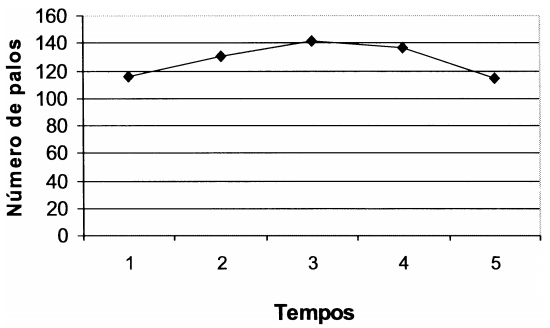
\includegraphics[width=0.76\textwidth]{./fig/grafico-rendimento/convexo}
 \caption{Rendimento convexo ou parabólico.}
  Fonte: \cite{psicohood2018}.
 \label{fig:convexo}
\end{figure}

\textbf{Côncavo} (NOR acima de 6): produção inicial mais alta, que diminui por uma falta de disposição durante a atividade
e recupera com a continuação da tarefa.

Ex.:
\begin{table}[h]
\centering
\caption{Rendimento côncavo\cite{psicohood2018} }
\label{tab:côncavo} 
\begin{tabular}{|l|c|c|c|c|c|c|}
\hline Tempos       & 1     & 2     & 3    &  4     & 5     & Total \\ 
\hline Nº de traços & 150 & 135 & 124 & 140 & 153 & 700 \\ 
\hline    \multicolumn{2}{|l|}{ Diferenças}& 15   & 11    &16     & 13    & 55\\ 
\hline NOR = 7,8\\
\cline{1-11}
\end{tabular} 

\end{table}

\begin{figure}[H]
 \centering
 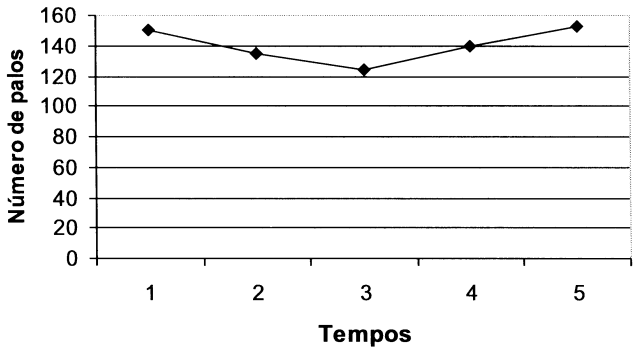
\includegraphics[width=0.76\textwidth]{./fig/grafico-rendimento/concavo}
 \caption{Rendimento côncavo.}
  Fonte: \cite{psicohood2018}.
 \label{fig:concavo}
\end{figure}

\textbf{Irregular ou oscilante }(NOR acima de 6): irregularidade no ritmo de trabalho, pode indicar estresse, falta de ânimo e disposição, motivação deficiente, ou interferência do estado emocional. Indica geralmente uma perturbação psíquica voluntária ou involuntária na administração do esforço.

Ex.:
\begin{table*}[h]
\centering
\caption{Rendimento irregular\cite{psicohood2018} }
\label{tab:irregular} 

\begin{tabular}{|l|c|c|c|c|c|c|}
\hline Tempos       & 1     & 2     & 3    &  4     & 5     & Total \\ 
\hline Nº de traços & 110 & 145 & 120 & 115 & 152 & 642 \\ 
\hline    \multicolumn{2}{|l|}{ Diferenças}& 35   & 25    &5     & 37    & 102\\ 
\hline NOR = 15,9\\
\cline{1-11}
\end{tabular} 

\end{table*}

\begin{figure}[H]
 \centering
 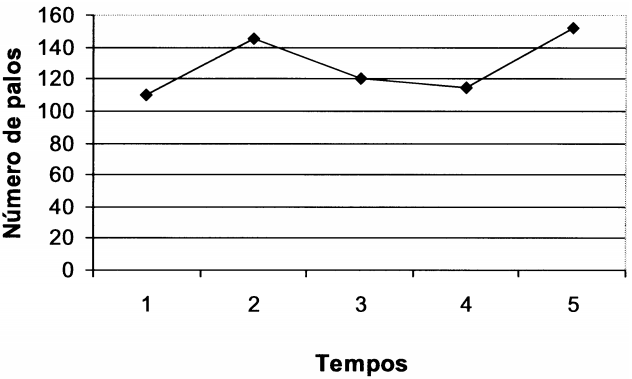
\includegraphics[width=0.76\textwidth]{./fig/grafico-rendimento/irregular}
 \caption{Rendimento irregular.}
  Fonte: \cite{psicohood2018}.
 \label{fig:irregular}
\end{figure}



\section{Visão computacional}
\label{sec:vc}
Visão computacional objetiva fazer com que os sistemas computacionais consigam enxergar, por meio da reprodução dos processos da visão humana utilizando software e hardware. Fazendo-se que o computador consiga realizar tarefas mais complexas e úteis na vida cotidiana e nos negócios como identificar doenças em raio-x, reconhecimento facial, ler sinais de trânsito, reconhecer pedestres, etc. \cite{dsAcademy2017}

Visão computacional é a combinação de várias técnicas de processamento de imagens  com o objetivo de identificar padrões, e reconhecer objetos em imagens. Ainda que a visão computacional já esteja sendo utilizada em diversas áreas de negócio, como no monitoramento de trânsito, identificar produtos e onde comprá-los, detecção de fraudes, reconhecimento de caracteres, monitoramento de fluxo de pessoas, identificação de pessoas entre outros. Ainda é uma tarefa muito complexa e está em evolução \cite{dsAcademy2017}.


Ensinar computadores a ver como os seres humanos é uma missão bem complexa, porque ainda não compreendemos por completo como o processo de visão realmente funciona \cite{dsAcademy2017}.

Conforme [Telles 2013 apud YANG 2007] é muito difícil criar sistemas de visão computacional que se assemelham  às  habilidades cognitivas dos  humanos, dentre as dificuldades estão a variação de iluminação, a dificuldade de generalizar objetos a partir de um conjunto pre-definido de imagens e as variações de posição do objeto em relação à câmera.

Diversos algorítimos foram desenvolvidos para extrair informações de imagens com a finalidade de automatizar tarefas na qual geralmente seriam feitas utilizando se da visão humana. Na visão humana  sabemos,  que  nossos olhos capturam as imagens e depois nosso cérebro realiza a análise e identificação do seu conteúdo. Na visão computacional realizamos uma série de etapas para reproduzir o processo da visão humana.

Dependendo do problema, todas as etapas explicadas a seguir são aplicadas, porém, isso não é uma regra, pode haver situações em que apenas algumas etapas já conseguem resolver o problema em questão utilizando-se de metologias diferentes  da apresentada.

Segundo \cite{digitalImgProcess2010} existem algumas etapas básicas na análise de dados em imagens que se dividem em: aquisição da imagem, pré-processamento, segmentação, descrição, reconhecimento e interpretação. Estas etapas estão englobadas em três áreas básicas: primeira, processamento de baixo nível, com funções que podem ser vistas como reações que não requerem comportamento inteligente; segunda processamento de nível intermediário, com extração e caracterização de componentes; e terceira processamento de alto nível, que utiliza-se de reconhecimento e interpretação. Na Figura \ref{fig:imgpdi} pode se ver todo esse processo.

\begin{figure}[H]
 \centering
 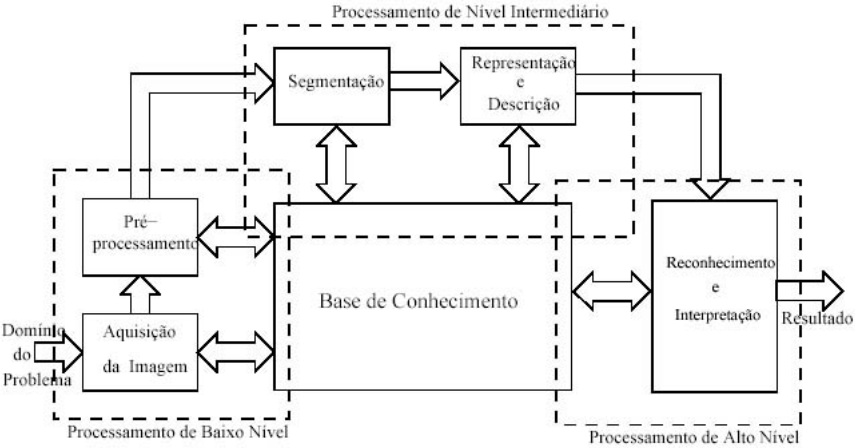
\includegraphics[width=0.89\textwidth]{./fig/fundamentacao/pdi2}
 \caption{Etapas de um sistema de visão computacional}
 \label{fig:imgpdi}
\end{figure}

Na etapa da aquisição da imagem acontece a captura e digitalização da imagem, por meio de um dispositivo de captura, nesse trabalho foi usado a câmera de um \textit{smartphone}. No pré-processamento, temos o tratamento da imagem, que pode ter vindo com ruídos e imperfeições intrínsecas da cena.  Na segmentação a imagem é dividida de acordo com as regiões de interesse, por exemplo os palos gravados na folha do teste. Na representação, são extraídas características relevantes ao domínio do problema e preparadas para o próximo passo. Na interpretação temos a atribuição de significado ao conjunto de objetos reconhecidos. 

\subsection{Aquisição de imagem}
\label{sub:aquis}

Existem diversos, dispositivos de captura de imagens, por exemplo, câmera, scanner, leitor biométrico, máquinas de raio-x, etc. A qualidade da imagem vai depender muito do dispositivo, e do ambiente onde esta sendo feito a aquisição, pois pode haver problemas, como falha mecânica do dispositivo, iluminação heterogênea, baixa resolução o que pode causar ruídos na imagem.

\subsection{Pré-processamento}
\label{sub:pre-process}

Nessa etapa, são aplicadas diversas operações tais como realce de contrastes, remoção de ruídos e suavização de regiões, melhorando a qualidade da mesma. Essas transformações são ditas de baixo nível, pois trabalham diretamente com os valores de intensidade de pixels, sem se importar nesse momento com informações relativas ao domínio do problema. O resultado é outra imagem de melhor qualidade que a original, isso aumenta as chances de sucesso dos processos seguintes [Filho & Neto, 1999].

Alguns exemplos de aplicação de filtros: a redução de ruídos, o controle do nível de brilho ou contraste, entre outras aplicações. 


\subsection{Segmentação}
\label{sub:segment}

Nesta etapa do pré-processamento a imagem é subdividida em partes de acordo com os objetos detectados na imagem. Cada uma dessas partes é uniforme e homogênea no tocante a algumas propriedades da imagem como textura e cor.

Os algoritmos de segmentação geralmente são baseados na busca pelas descontinuidades ou pelas similaridades dos níveis de cinza. \cite{digitalImgProcess2010} O objetivo da segmentação é agrupar um conjunto de pixels de mesma propriedade, para isso, não pode haver erro, pois isso pode comprometer o sucesso da análise da imagem.

Na descontinuidade, o particionamento da imagem é baseado no subconjunto de pontos de um objeto que o separa do restante da imagem, quer dizer, são representadas por alterações abruptas nos tons de cinza, cores e texturas. Na similaridade, a segmentação é baseada nos aspectos comuns dos pixels da imagem, inicialmente, o método começa com um pixel, e a partir deste pixel, examina-se seus vizinhos, numa determinada sequência, para decidir se eles possuem níveis de cinza similares, segundo o critério de similaridade escolhido, existem diversas técnicas de segmentação por similaridade,  uma delas é a limiarização a qual foi utilizada nesse trabalho.


\subsection{Representação e descrição}
\label{sub:rep-desc}

Após a etapa de segmentação é obtido um agregado de pixels segmentados. Pode ser necessário transformar os dados para uma forma adequada para o futuro processamento por computador. Neste caso podem ser utilizadas as representações por características externas (sua fronteira) ou características internas (os pixels que constituem a região). A representação por fronteira é adequada quando o foco está em características externas da forma,  por exemplo, em cantos. Uma representação por região é apropriada quando o foco está em propriedades internas do objeto como forma, cor ou textura. Dependendo do projeto é necessário usar às duas categorias de representação. Escolher a representação é apenas parte da solução para a transformação de dados brutos em uma forma conveniente para o processamento na próxima etapa. Um método para descrever os dados deve ser especificado, de maneira que as características de interesse sejam enfatizadas. Descrição, é utilizada na extração de atributos que tem como resultado, informação quantitativa ou que possa ser utilizada para diferenciar classes de objetos \cite{digitalImgProcess2010}.

Estes descritores devem ser representados por uma estrutura de dados adequada ao algoritmo de reconhecimento. Nessa etapa a entrada ainda é uma imagem, mas a saída é uma lista de dados correspondentes a imagem. Por exemplo, os descritores utilizados nesse trabalho para os descrever os palos foram as coordenadas x e y sua área, altura, largura e sua forma retangular. Neste caso, um vetor armazena essas características em seguida cada vetor é adicionado em um lista de dados. 

\subsection{Reconhecimento e interpretação}
\label{sub:rec-intr}

O reconhecimento faz a atribuição de rótulo a um objeto (por exemplo, “veículo”), tendo como base as informações fornecidas na etapa anterior pelo descritor e a interpretação atribui um significado a um conjunto de objetos reconhecidos. No exemplo de reconhecimento de caracteres, este passo seria responsável por identificar que um determinado conjunto de objetos, por exemplo, cinco números seguidos por um hífen e outros três números representa um CEP. O reconhecimento sobre o domínio do problema está codificado em sistema de processamento de imagens na forma de uma base de conhecimento. Este pode ser simples quanto o detalhamento de regiões de uma imagem na qual se sabe que a informação de interesse pode ser localizada, ou complexa, por exemplo, uma lista inter-relacionada de todos os principais defeitos possíveis em um problema de inspeção de materiais, isso vai depender do domínio do problema.\cite{digitalImgProcess2010}


\section{Imagem Digital}
\label{sec:img}

Uma imagem digital é representada por um matriz de linhas e colunas que definem cada ponto(x,y) na imagem. Cada ponto na matriz bidimensional é denominado pixel. Os pontos são coordenadas espaciais onde as linhas y e colunas x são definidos por um função bidimensional f(x,y), que corresponde ao valor do elemento e a intensidade do nível de cinza ou cor naquele ponto da matriz. Quando (x, y) e os valores de intensidade f são quantidades finitas e discretas, temos a imagem digital. \cite{ImgDigital2001} 

Na figura \ref{fig:imgDigital} temos uma imagem monocromática identificando sua origem  (0,0) e a posição dos eixos no plano cartesiano.

\begin{figure}[H]
 \centering
 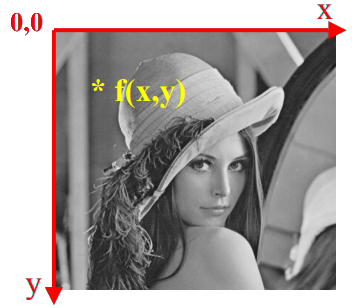
\includegraphics[width=0.60\textwidth]{./fig/fundamentacao/lenna}
 \caption{Demostração de uma Imagem digital}
  Fonte: \cite{imagemDigital2019}.
 \label{fig:imgDigital}
\end{figure}


\subsection{Sistemas de cores}
\label{sub:siscores}

\subsubsection{Escala de cinza}
\label{subsub:siscores-cinza}

A luz quando sem cor é chamada monocromática. A intensidade da luz monocromática pode variar entre o preto (0) , passando por tons de cinza, até o branco (255), chamado de nível de cinza. Essa variação na intensidade é conhecida por escala de cinza. 
Essa escala de cinza possui uma variação de 256 tonalidades, pois possuem 8 bits para representarem essas tonalidades. 

Para diminuir o peso do processamento da imagem, antes de qualquer operação, as imagens devem ser convertidas para escala de cinza.\cite{digitalImgProcess2010}


\subsubsection{Sistema de cores RGB}
\label{subsub:siscores-RGB}

O padrão de cores RGB trabalha com as cores   vermelho (\textit{Red}), verde (\textit{Green}) e  azul(\textit{Blue}). Cada uma dessas cores possui uma variação de 256 valores.  Cada cor pode receber um valor de intensidade de 0 até 255, e podem ser combinadas gerando mais de 16,7 milhões de cores distintas.  A Figura  \ref{fig:imgCORES} mostra um exemplo de combinações das cores RGB.  Neste trabalho foi utilizado a biblioteca Opencv que trabalha com a imagem no padrão BGR, a diferença é somente a ordem das cores.

\begin{figure}[H]
 \centering
 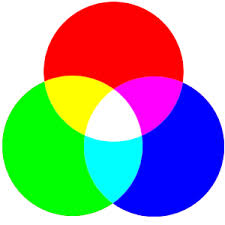
\includegraphics[width=0.30\textwidth]{./fig/fundamentacao/cores-rgb}
 \caption{cores RGB}
 Fonte: \cite{coresRGB}.
 \label{fig:imgCORES}
\end{figure}

\subsubsection{Sistema de cores HSV}
\label{subsub:siscores-HSV}


HSV é abreviatura para os componentes de tom (\textit{hue}), saturação (\textit{saturation}) e valor (\textit{value}). Este sistema é conhecido também como HSB (\textit{hue, saturation, brightness}). 
\textit{Hue} :  é o tipo de cor ou tonalidade, pode ser vermelho, amarelo, azul, etc. Pode ter valores entre 0 e 360, mas para algumas aplicações, este valor é normalizado de 0 a 100\%.
\textit{Saturation} : determina a profundidade ou pureza da cor (de esmaecida a intensa) Pode ter valores entre 0 e 100\% sendo mais saturada aquela mais próxima ao 100\%.
\textit{Value}: determina a intensidade percebida ( cor mais clara ou mais escura)
na Figura \ref{fig:imgHSV} é mostrado a representação desse sistema.

\begin{figure}[H]
 \centering
 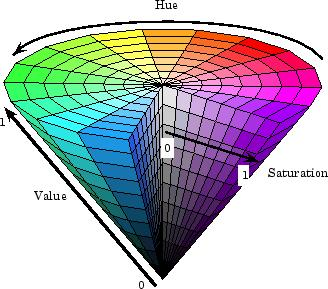
\includegraphics[width=0.30\textwidth]{./fig/fundamentacao/hsvcone}
 \caption{cores HSV}
 Fonte: \cite{coresHSV}
 \label{fig:imgHSV}
\end{figure}

\section{Histograma}
\label{sec:histograma}

No processamento de imagem o histograma calcula quantos pixels existem naquela tonalidade. Estes valores são geralmente representados por um gráfico de barras no qual cada retângulo representa um intervalo e sua altura representa a frequência naquele intervalo través do histograma.
Com a imagem em escala de cinza o histograma representa a distribuição dos níveis de cinza da imagem. O histograma possibilita um melhor entendimento da qualidade da imagem como nível de contraste e seu brilho. \cite{ImgDigital2001}

Na Figura \ref{subfig:histograma} tem a representação dos histogramas de quatro imagens básicas.
\begin{figure}[h]
 \centering
  \subfigure[][Imagem escura.]
   {
    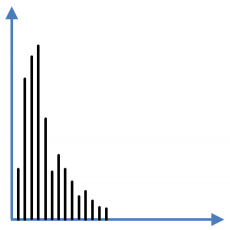
\includegraphics[width=0.22\textwidth]{./fig/fundamentacao/a}
    \label{subfig:hist-a}
   } \qquad
    \subfigure[][Imagem clara.]
   {
    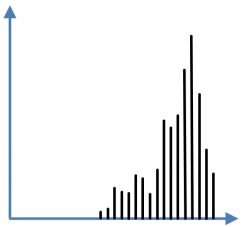
\includegraphics[width=0.22\textwidth]{./fig/fundamentacao/b}
    \label{subfig:hist-b}
   } \qquad
   \subfigure[][Imagem de baixo contraste.]
   {
    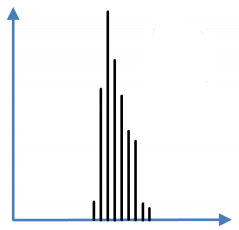
\includegraphics[width=0.22\textwidth]{./fig/fundamentacao/c}
    \label{subfig:hist-c}
   } \qquad
  \subfigure[Imagem de alto contraste.]
   {
    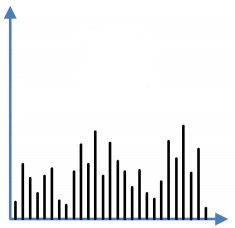
\includegraphics[width=0.22\textwidth]{./fig/fundamentacao/d}
    \label{subfig:hist-d}
   }
   \caption{{\subref{subfig:hist-a}} , {\subref{subfig:hist-b}}, {\subref{subfig:hist-c}} e {\subref{subfig:hist-d}} Histogramas referentes a quatro tipos básicos de imagens \cite{digitalImgProcess2010} }
  \label{subfig:histograma}
\end{figure}


\subsection{Equalização do Histograma}
\label{sub:equa-hist}

A equalização do histograma procura redistribuir os valores dos níveis de cinza na imagem, para se obter um histograma uniforme, no qual o número de pixels de qualquer nível é praticamente o mesmo, isso melhora o contraste da imagem.
É utilizado para corrigir problemas de contraste na imagem monocromática, causados por iluminação deficiente, excessiva ou mesmo de calibração incorreta do obturador. Essa técnica também podem ser aplicada a partes da imagem, em janelas m x n, para realçar detalhes minuciosos de pequenas porções da imagem \cite{pdi99}.

A Figura \ref{subfig:equl-histograma} apresenta um exemplo de aplicação da técnica de equalização de histograma
para aumentar o contraste de uma imagem 446 x 297 com 256 tons de cinza \cite{pdi99}.

\begin{figure}[h]
 \centering
  \subfigure[][Imagem original.]
   {
    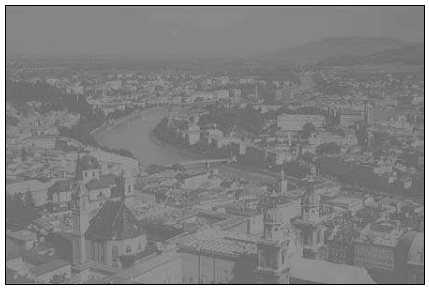
\includegraphics[width=0.30\textwidth]{./fig/fundamentacao/hist-a}
    \label{subfig:histi-a}
   } \qquad
    \subfigure[][Histograma da imagem original.]
   {
    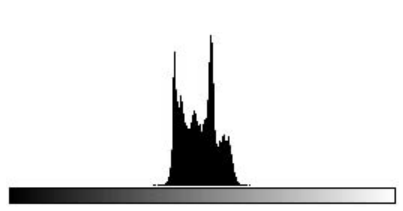
\includegraphics[width=0.30\textwidth]{./fig/fundamentacao/hist-grafico-b}
    \label{subfig:hist-grafico-b}
   } \qquad
   \subfigure[][Imagem equalizada.]
   {
    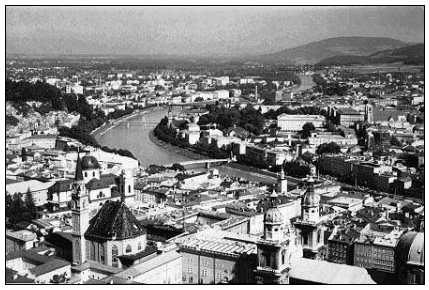
\includegraphics[width=0.30\textwidth]{./fig/fundamentacao/hist-equl-c}
    \label{subfig:histi-c}
   } \qquad
  \subfigure[Histograma da imagem equalizada.]
   {
    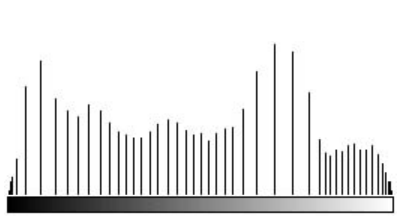
\includegraphics[width=0.30\textwidth]{./fig/fundamentacao/hist-grafico-d}
    \label{subfig:hist-grafico-d}
   }
   \caption{ Aplicação da equalização de histograma a imagens com baixo contraste \cite{pdi99}}
  \label{subfig:equl-histograma}
\end{figure}



\section{Limiarização }
\label{sec:limiar}

O limiarização (\textit{Thresholding}) tem como objetivo dividir uma imagem em regiões separando fundo e o objeto, tendo como base a análise de níveis de cinza em relação a um limiar T. Esse processo transforma uma imagem de escala de cinza para uma com pixels pretos e brancos, essa transformação consiste em comparar cada pixel da imagem com o valor do limiar T, qualquer ponto (x,y) na imagem em que f(x,y) > T esse ponto recebera o valor \textbf{1} identificando como sendo do objeto e caso contrário, o ponto receberá o valor \textbf{0} este será o fundo (background) da imagem, tendo como saída uma imagem binária g(x,y) \cite{digitalImgProcess2010}.

\begin{center}
    $g(x,y)= \left\{\begin{matrix}
        & 1 \ se \  \textit{f}(x,y) > T   \\ 
        & 0 \ se \  \textit{f}(x,y) \leq  T
    \end{matrix}\right\\$ 
\end{center} 

Por convenção são utilizados os valores de intensidade 0 e 1, mas podem ser utilizados dois valores quaisquer, desde que sejam distintos. A definição de um bom limiar é essencial para o que processo de limiarização seja satisfatório. Devido às variações de brilho e contraste, a definição de um limiar não é simples. 

Existem diversas variantes de limiarização a mais simples define o seu limiar único T baseado na análise do histograma da imagem. Na Figura \ref{subfig:limiarizacao} pode se ver um exemplo de definição de limiar baseado no histograma, na imagem temos dois picos e um vale um caso de limiarização mais simples \cite{pdi99}.

\begin{figure}[h]
 \centering
   \subfigure[][Histograma original.]
   {
    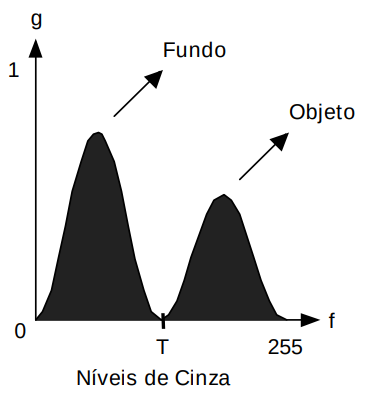
\includegraphics[width=0.22\textwidth]{./fig/fundamentacao/hist-cinza}
    \label{subfig:hist-cinza}
   } \qquad
  \subfigure[Histograma da imagem binarizada.]
   {
    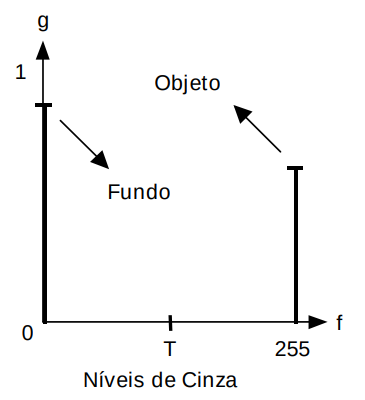
\includegraphics[width=0.22\textwidth]{./fig/fundamentacao/hist-bin}
    \label{subfig:hist-bin}
   }
   \caption{ Limiarização de uma imagem monocromática utilizando limiar T. \cite{pdi99}}
  \label{subfig:limiarizacao}
\end{figure}

Quando o limiar T é aplicado na imagem inteira temos a limiarização global e quando esse limiar T depende de propriedades de pixels de uma vizinhança ou de coordenadas espaciais(x,y) temos a limiarização adaptativa ou dinâmica.\cite{digitalImgProcess2010}

A limiarização é muito importante para o sucesso na segmentação de objetos na imagem.

\section{Filtro espacial de suavização (\textit{blur})}
\label{sec:blur}

O filtro de suavização ou borramento, tem a função de embaçamento na imagem, diminuindo a definição, contribuindo para a redução de ruídos. Esse filtro normalmente é usado no pré-processamento para a segmentação de objeto e conexão de pequenas descontinuidades em linhas ou curvas.\cite{digitalImgProcess2010}

A suavização é obtida pela média dos pixels vizinhos tendo como base uma máscara. Esse filtro de suavização também é conhecido como filtro passa baixa. A suavização elimina mudanças bruscas na intensidade entre os pixels, causando perca de nitidez reduzindo assim os ruídos, porém deve-se ter cuidado, pois isso pode prejudicar a detecção de bordas.

Na figura \ref{subfig:suavizacao}, é apresentado a aplicação de suavização de uma imagem.

\begin{figure}[h]
 \centering
   \subfigure[][Imagem original.]
   {
    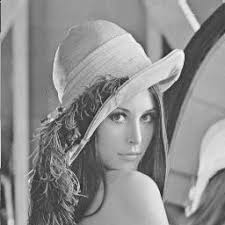
\includegraphics[width=0.26\textwidth]{./fig/fundamentacao/lenna-gray}
    \label{subfig:blur-original}
   } \qquad
   \subfigure[][Imagem suavizada com máscara 3x3.]
   {
    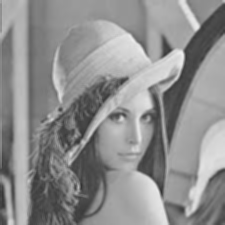
\includegraphics[width=0.26\textwidth]{./fig/fundamentacao/lenna-blur-3}
    \label{subfig:blur-3}
   } \qquad
  \subfigure[Imagem suavizada com máscara 5x5.]
   {
    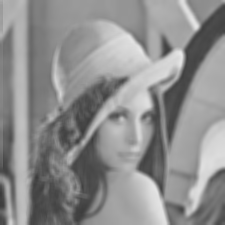
\includegraphics[width=0.26\textwidth]{./fig/fundamentacao/lenna-blur-5}
    \label{subfig:blur-5}
   }
   \caption{ Aplicação do filtro da média com mascara 3x3 e 5x5.}
      Fonte: \cite{imagemDigital2019}
  \label{subfig:suavizacao}
\end{figure}

\section{Detecção de bordas}
\label{sec:bordas}

Bordas(\textit{\textbf{edges}}) podem ser definidas como o limite entre duas regiões cujos níveis de cinza sofrem uma mudança bruta de brilho na imagem. As bordas são os contornos dos objetos, e são muito importantes para identificar e segmentar objetos em imagens.\cite{digitalImgProcess2010}

As bordas são utilizadas com mais frequência do que detecção de pontos e linhas, apesar de que pontos e linhas isolados também são utilizados em segmentação, porém,  não são muito frequentes em aplicações práticas. \cite{digitalImgProcess2010}

O reconhecimento de bordas não é trivial, devido a problemas como variação na iluminação, um objeto atrás do outro que geralmente será mais escuro; um objeto perpendicular à iluminação é mais claro que um que esteja paralelo; mudanças das propriedades de material, textura e cor; características como reflexão e refração tudo isso é um grande desafio na detecção de bordas. 

Existem diversas técnicas para detecção de borda uma delas é a utilização  de operadores diferenciais com uso de máscaras de convolução. Esses operadores encontram as variações nos níveis de pixels com a aplicação das derivadas primeira e segunda. Consegue-se detectar as bordas fazendo a convolução da máscara  para cada pixel na imagem.\cite{digitalImgProcess2010}

Neste trabalho foram testados dois operadores o Canny e o Sobel sendo o Sobel o que apresentou um melhor resultado.
O Sobel utiliza o gradiente para a determinação da borda na imagem. A Figura \ref{subfig:mascara-sobel} ilustra as máscaras utilizadas pelo operador Sobel na detecção de bordas horizontais e verticais.

\begin{figure}[h]
 \centering
   \subfigure[][Máscara horizontal.]
   {
    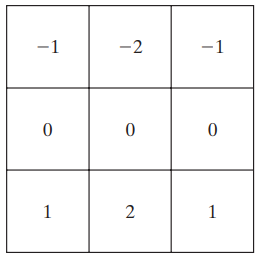
\includegraphics[width=0.20\textwidth]{./fig/fundamentacao/m-sobel-h}
    \label{subfig:blur-original}
   } \qquad
   \subfigure[][Máscara Vertical.]
   {
    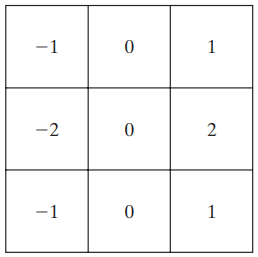
\includegraphics[width=0.20\textwidth]{./fig/fundamentacao/m-sobel-v}
    \label{subfig:blur-3}
   } \qquad
  \subfigure[Máscara de posição.]
   {
    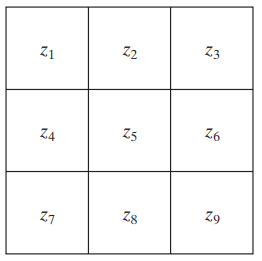
\includegraphics[width=0.20\textwidth]{./fig/fundamentacao/m-sobel-z}
    \label{subfig:blur-5}
   }
   \caption{ Máscaras utilizadas no operador Sobel. \cite{digitalImgProcess2010}}
  \label{subfig:mascara-sobel}
\end{figure}

As derivadas aplicadas nas máscaras do operador de Sobel são mostradas nas equações (1) e (2). Por meio delas consegue-se estimar a presença de mudança de região  de tons claros e escuros.

\ (1) 
\begin{center}
    $g(x)=\frac{\partial f(x,y)}{\partial x}=(Z_{7}+2Z_{8}+Z_{9})-(Z_{1}+2Z_{2}+Z_{3})$ 
\end{center}

\ (2)
\begin{center}
    $g(y)=\frac{\partial f(x,y)}{\partial y}=(Z_{3}+2Z_{6}+Z_{9})-(Z_{1}+2Z_{4}+Z_{7})$ 
\end{center}

Para cada ponto da imagem  é calculada na equação (3) a aproximação do gradiente combinando o resultado (1) e (2).

\ (3)
\begin{center}
    $G=\sqrt{g(x)^{2} + g(y)^{2}}$
\end{center}

O resultado do deslocamento das máscaras para todos os pixel é uma de gradiente com as mesmas dimensões da original. \cite{digitalImgProcess2010}

Na figura \ref{subfig:filtro-sobel} vemos a aplicação do filtro Sobel.

\begin{figure}[h]
 \centering
   \subfigure[][Imagem original.]
   {
    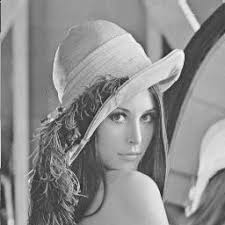
\includegraphics[width=0.25\textwidth]{./fig/fundamentacao/lenna-gray}
    \label{subfig:sobel-original}
   } 
   \qquad
  \subfigure[Imagem com filtro de Sobel.]
   {
    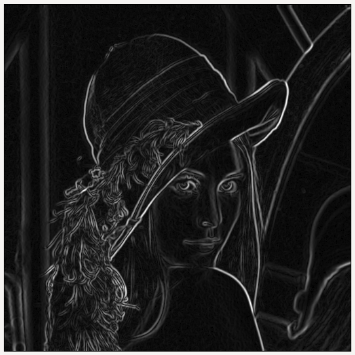
\includegraphics[width=0.25\textwidth]{./fig/fundamentacao/lenna-sobel}
    \label{subfig:sobel-filtro}
   }
   \caption{ Aplicação do filtro de Sobel para detectar bordas.}
  \label{subfig:filtro-sobel}
\end{figure}

\section{Morfologia Matemática}
\label{sec:morfologia}
A morfologia matemática tem em sua essência extrair informações relativas à geometria e à topologia de uma imagem, realizando transformações por um elemento estruturante. Algumas das aplicações dessa técnica no processamento de imagens são:  realce, filtragem, segmentação, detecção de bordas, esqueletização e afinamento de imagens. \cite{pdi99} Neste trabalho foram utilizadas duas operações fundamentais da morfologia matemática a dilatação e a erosão.

Na erosão os pixels que formam um determinado padrão são retirados da imagem, e na dilatação é ao contrário os pixels são adicionados à imagem de acordo com a forma do elemento estruturante escolhido.\cite{digitalImgProcess2010}

A técnica de operações morfológicas é baseada na teoria dos conjuntos, na qual os conjuntos representam a forma dos objetos em uma imagem. Em imagens binárias os conjuntos de pixels pertencem ao espaço bidimencional inteiro $Z^{2}$ e cada elemento do conjunto é um vetor 2-D, cujas coordenadas (x,y) representam os pixels pretos (por convenção) na imagem.\cite{pdi99}

\subsection{Dilatação}
\label{subsec:morfologia-dila}

Sejam A e B conjuntos no espaço $Z^{2}$ o processo de dilatação se baseia na reflexão\footnote{ Na reflexão, todos os elementos de B em torno da origem desse conjunto são refletidos. Representada por $\hat{B}$ é simplesmente o conjunto dos pontos em B cujas coordenadas (x,y) foram substituídas por (-x,-y) }  de B em torno de sua origem e depois deslocar esta reflexão de x. A dilatação de A por B é, então, o conjunto de todos os x deslocamentos para os quais a interseção de $(\hat{B})_{x}$ e A influi pelo menos um elemento diferente de zero. Com base nesta interpretação, temos a seguinte equação, sendo B o elemento estruturante (ES).\cite{pdi99}

\begin{center}
    $A \oplus B = \begin{Bmatrix}
    x\mid \left [ (\hat{B})_{x}\cap A \right  ] \subseteq A 
    \end{Bmatrix}$
\end{center}

A dilação diferentemente da erosão provoca o engrossamento dos objetos na imagem, de acordo com o elemento estruturante escolhido. Na figura \ref{subfig:dilatacao} temos um exemplo de dilatação, onde no centro temos o elemento estruturante que vai percorrer a imagem, e cada vez que seu pixel central coincidir com o mesmo pixel na imagem original, o elemento estruturante é inserido na imagem tendo como resultado uma imagem dilatada.

\begin{figure}[h]
 \centering
  \subfigure[Imagem original \textbf{A}]
   {
    
\includegraphics[width=0.20\textwidth]{./fig/fundamentacao/a-dilat}
     \label{subfig:a-dilat}
   }
   \qquad
  \subfigure[ES \textbf{B = $\hat{\textbf{B}}$}]
   {
    
\includegraphics[width=0.10\textwidth]{./fig/fundamentacao/e-dilat}
    \label{subfig:e-dilat}
   }
   \qquad
  \subfigure[Resultado da dilatação \textbf{A $\oplus$ B }]
   {
    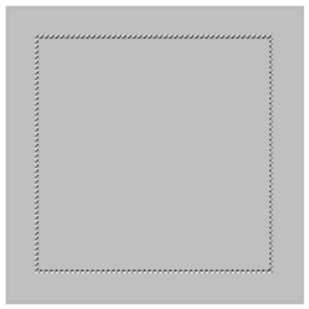
\includegraphics[width=0.25\textwidth]{./fig/fundamentacao/ab-dilat}
    \label{subfig:ab-dilat}
   }
   \caption{ Exemplo de dilatação. \cite{pdi99}}
  \label{subfig:dilatacao}
\end{figure}

\subsection{Erosão}
\label{subsec:morfologia-erosao}

A erosão provoca o afinamento do objeto na imagem binária, sendo que elementos menores que o elemento estruturante, incluindo pontos isolados, são removidos contribuindo para a remoção de ruídos. \cite{digitalImgProcess2010}

Sendo A e B como conjunto de $Z^{2}$, temos que a erosão de A por B indicada por A $\ominus$ B,  é o conjunto de todos os pontos x de forma que B, transladado \footnote{A translação na matemática é o movimento de um elemento de um ponto a outro. É análoga à operação de rotacionar } de x, está contido em A. Assim sendo A representa o objeto na imagem e B o elemento estruturante. Por B estar contido em A, o elemento estruturante não em comum com o fundo, sendo $A^{c}$ o complemento do conjunto A, ou seja, o fundo da imagem, então a erosão pode ser expressa com a seguinte equação:
\cite{pdi99}

\begin{center}
    $A \ominus  B = \begin{Bmatrix}
    x\mid   (B)_{x}\cap A^{c}    =  \varnothing 
    \end{Bmatrix} $
\end{center}

A diferença da erosão para a dilatação é que quando o pixel central do elemento estruturante coincide com o da imagem, ao invés de acrescentar os pixels desse elemento, esses são retirados da imagem. Então a imagem resultante será menor que a original sofrendo a erosão. Na Figura \ref{subfig:dilatacao} temos o exemplo de erosão.

\begin{figure}[h]
 \centering
  \subfigure[Imagem original \textbf{A}]
   {
    
\includegraphics[width=0.25\textwidth]{./fig/fundamentacao/a-dilat}
     \label{subfig:a-dilat}
   }
   \qquad
  \subfigure[ ES \textbf{ B = $\hat{\textbf{B}}$}]
   {
    
\includegraphics[width=0.10\textwidth]{./fig/fundamentacao/e-dilat}
    \label{subfig:e-dilat}
   }
   \qquad
  \subfigure[Resultado da erosão \textbf{A $\ominus$ B }]
   {
    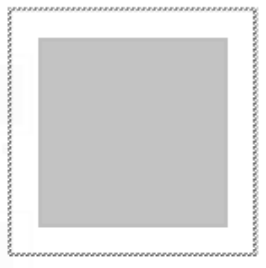
\includegraphics[width=0.25\textwidth]{./fig/fundamentacao/ab-erosao}
    \label{subfig:ab-dilat}
   }
   \caption{ Exemplo de erosão. \cite{pdi99}}
  \label{subfig:dilatacao}
\end{figure}
 \chapter{Desenvolvimento}
\label{cap:desenv}

% - - - - - - - - - - - - - - - - - - - - - - - - - - - - - - - - - - -
\section{Abordagem Inicial}
\label{sec:abord-ini} 
Neste capítulo será abordado todos os passos realizados para se alcançar o objetivo esperado deste trabalho. Para desenvolvimento foi utilizado a linguagem de programação Python por  ter sintaxe simples e suporte a biblioteca OPenCV (\textit{Open Source Computer Vision}) a qual possui diversas técnicas eficientes  e robustas voltadas para processamento de imagens, visão computacional e com  foco em aplicações em tempo real.

Neste trabalho foi utilizado para captura das imagens um iphone 5 resolução da câmera ( 3264 x 2448 pixel) e posteriormente um 6s (4608 x 2592 pixel). A ideia é que, futuramente esse protótipo possa funcionar em qualquer smartphone sem a necessidade de compra de um hardware especial como acontece em \cite{skip2018} que utiliza scanners específicos para ler os palos.

A abordagem deste trabalho é direcionada na utilização de algoritmos de processamento de imagens e visão computacional para ler uma imagem de um teste palográfico e realizar a contagem dos palos, disponibilizando uma análise quantitativa em tempo real, otimizando o trabalho de correção dos testes.

\section{Visão geral do protótipo}
\label{sec:visao-geral}

Os passos de execução  do algoritmo segue a seguinte ordem:
Carregar a Imagem, Localização da folha, Pré-processamento, Segmentação, Identificação dos palos e Contagem. A Figura \ref{fig:visao-geral} mostra esse processo.

\begin{figure}[H]
 \centering
 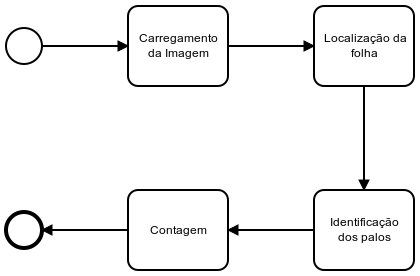
\includegraphics[width=0.76\textwidth]{./fig/desenvolvimento/visao-geral}
 \caption{Fluxo do processo para contagem dos palos.}
 \label{fig:visao-geral}
\end{figure}

Na etapa de carregamento a imagem que contém o teste palográfico é carregada na memória e redimensionada, em seguida é repassada para a o pré-processamento e segmentação no qual são aplicados filtros e transformações na imagem para facilitar na etapa de localização  da folha nessa etapa é feito a separação dos objetos  do fundo da imagem e extração do ROI(Região de Interesse) que é a nossa folha do teste palográfico na próxima etapa é aplicado novamente o pré-processamento e segmentação porém dessa vez somente na ROI onde são extraídos os objetos em forma de retângulos que são adicionados em uma lista e repassados para a fase de identificação dos palos onde são feitas validações para identificar os palos. 

No final é feito a contagem dos palos na ordem considerando o intervalo dos 5 tempos. Nas seções seguintes será abordado com mais detalhes os processos descritos.

\section{Carregamento da imagem}
\label{sec:carrega-imagem}
Este trabalho tem o propósito de contar os palos em uma imagem capturada por celular, no entanto, não será desenvolvido nenhum aplicativo para celular apenas o algoritmo de visão computacional para realizar a contagem. Neste protótipo as imagens capturadas pelo celular são transferidas para o computador para serem utilizadas no algoritmo. 


\begin{figure}[H]
 \centering
 
\includegraphics[width=0.83\textwidth]{./fig/desenvolvimento/teste-palos}
 \caption{Exemplo de teste palográfico capturado por celular.}
 \label{fig:ex-teste-palo}
\end{figure}


\subsection{Restrições}
\label{subsec:restricoes}
Para o funcionamento correto do protótipo alguns cuidados devem ser tomados na captura das imagens, não utilizar o flash do celular, pois isso gera uma imagem com uma luz mais forte em um só ponto, prejudicando o processamento da imagem. A imagem deve ter uma iluminação homogênea como na Figura \ref{fig:ex-teste-palo}, também deve se tomar cuidado para não fazer sombra sobre a imagem e não amassar e nem dobrar a folha do teste.

\section{Localização da folha}
\label{sec:loc-folha}

Nessa etapa para localizar a região onde se encontra a folha com o teste dos palos na imagem foi utilizado diversas técnicas de processamento de imagens. 

\subsection{Pré-processamento}
\label{sec:pre-proce}

Após o carregamento da imagem é aplicado o filtro Gaussiano para redução de ruídos depois é  feito a conversão para o formata HSV, em seguida é feito uma divisão separando as camadas de Tonalidade(\textit{Hue}), Saturação (\textit{Saturation}) e  Brilho (\textit{Value}) da imagem. Na Figura  \ref{fig:subfiguras} pode ser visto a aplicação dessas técnicas.
\begin{figure}[h]
 \centering
  \subfigure[][Exemplo de conversão da imagem para HSV.]
   {
    
    \includegraphics[width=0.25\textwidth]{./fig/desenvolvimento/hsv_x_orig}
    \label{subfig:ex1}
   } \qquad
  \subfigure[Split da imagem separando as camadas Hue, Saturation e Value]
   {
    \includegraphics[width=0.37\textwidth]{./fig/desenvolvimento/hsv_split}
    \label{subfig:ex2}
   }
   \caption{{\subref{subfig:ex1}} e {\subref{subfig:ex2}} Resultado do processamento da imagem nessa etapa inicial }
  \label{fig:subfiguras}
\end{figure}
No passo seguinte é aplicado uma transformação morfológica na parte Saturada da imagem,  chamada \textit{Closing} que é uma dilatação seguida de uma erosão. Foi utilizado como teste diversas transformações morfológicas, porém essa foi a que mostrou melhor resultado. Foi realizado uma limiarização (ou binarização) responsável por localizar os objetos presentes na imagem, para isso foram feitos testes com as funções \textbf{threshold} e \textbf{adaptativeThreshold} nativas da biblioteca \textbf{Opencv}, foi obtido  melhor resultado com a função \textbf{adaptativeThreshold}, por trabalhar melhor em imagens com iluminação variável. Os parâmeros utilizados na função foram 255 para o valor máximo, \textbf{ADATIVE THRESH GAUSSIAN C}  para o método, tipo de limiarização \textbf{THRESH BINARY}, 111 para \textbf{Block Size } e 13 para a constante \textbf{C}.
O resultado pode ser visto na Figura  \ref{subfig:adp-thres} 

\begin{figure}[h]
 \centering
  \subfigure[][Imagem binarizada pela função adaptative threshold.]
   {
    
    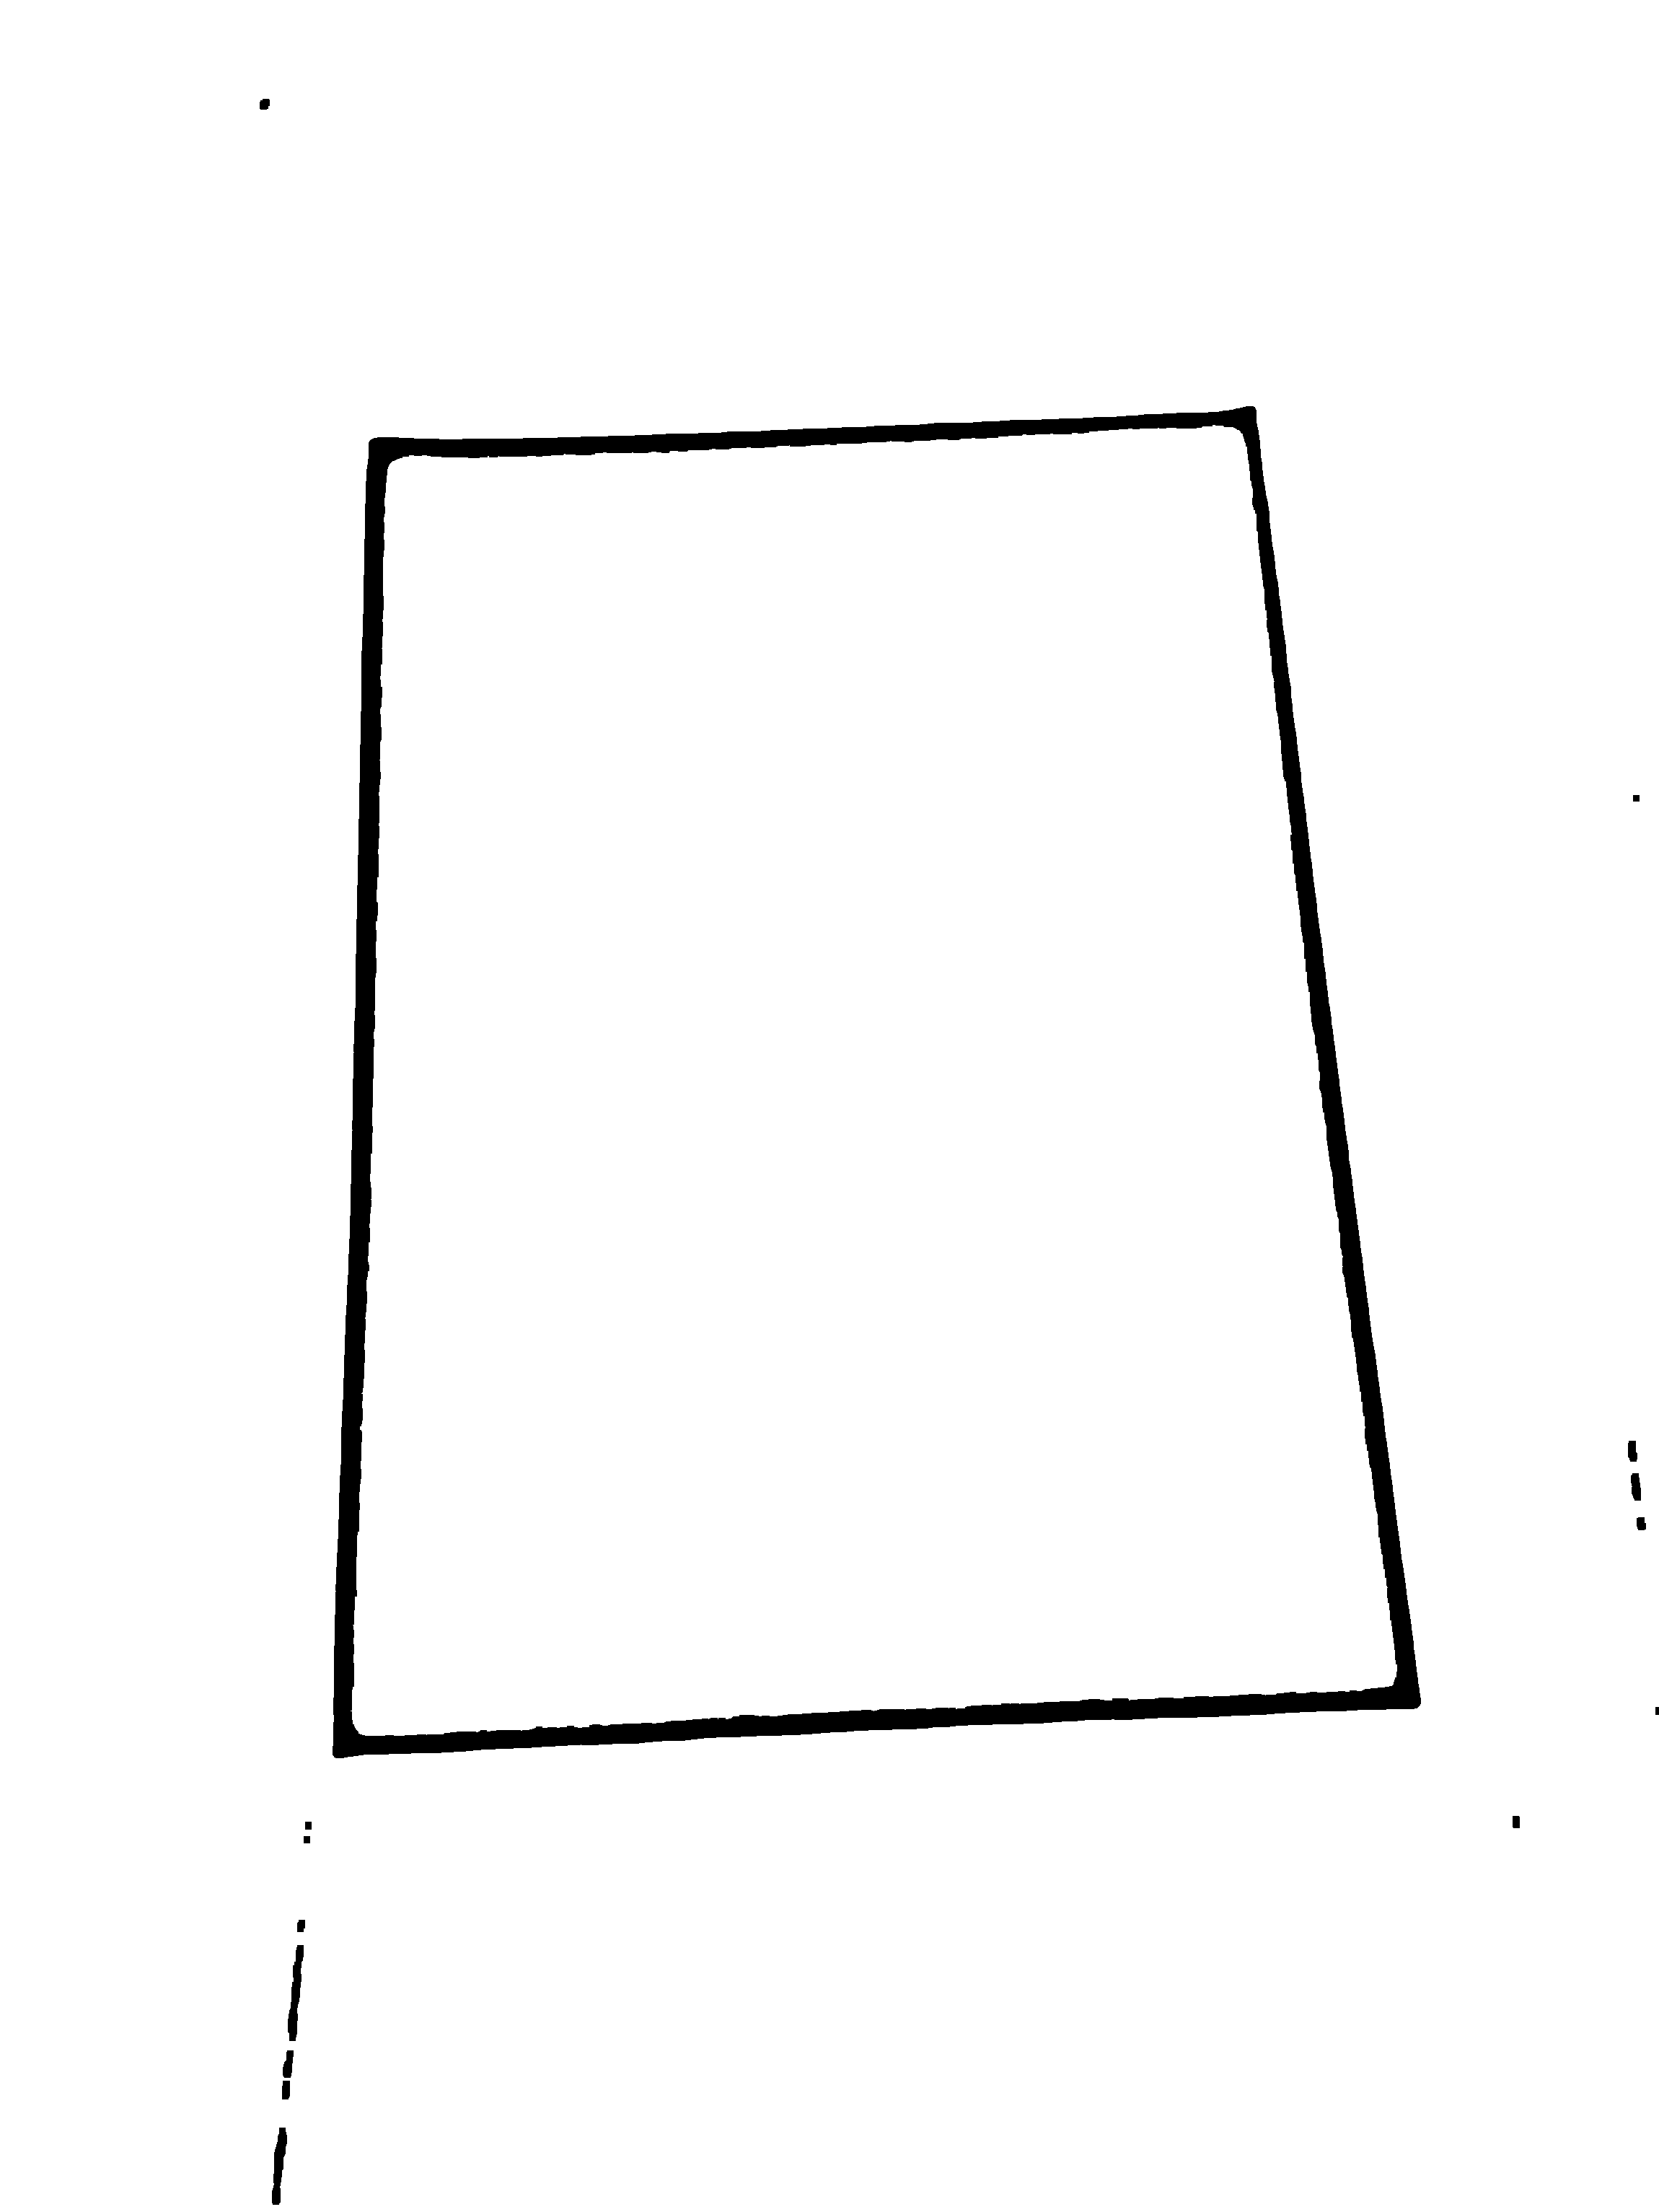
\includegraphics[width=0.37\textwidth]{./fig/desenvolvimento//adaptative_thres}
    \label{subfig:adp-thres}
   } \qquad
  \subfigure[Detecção de bordas usando o algoritmo Sobel]
   {
    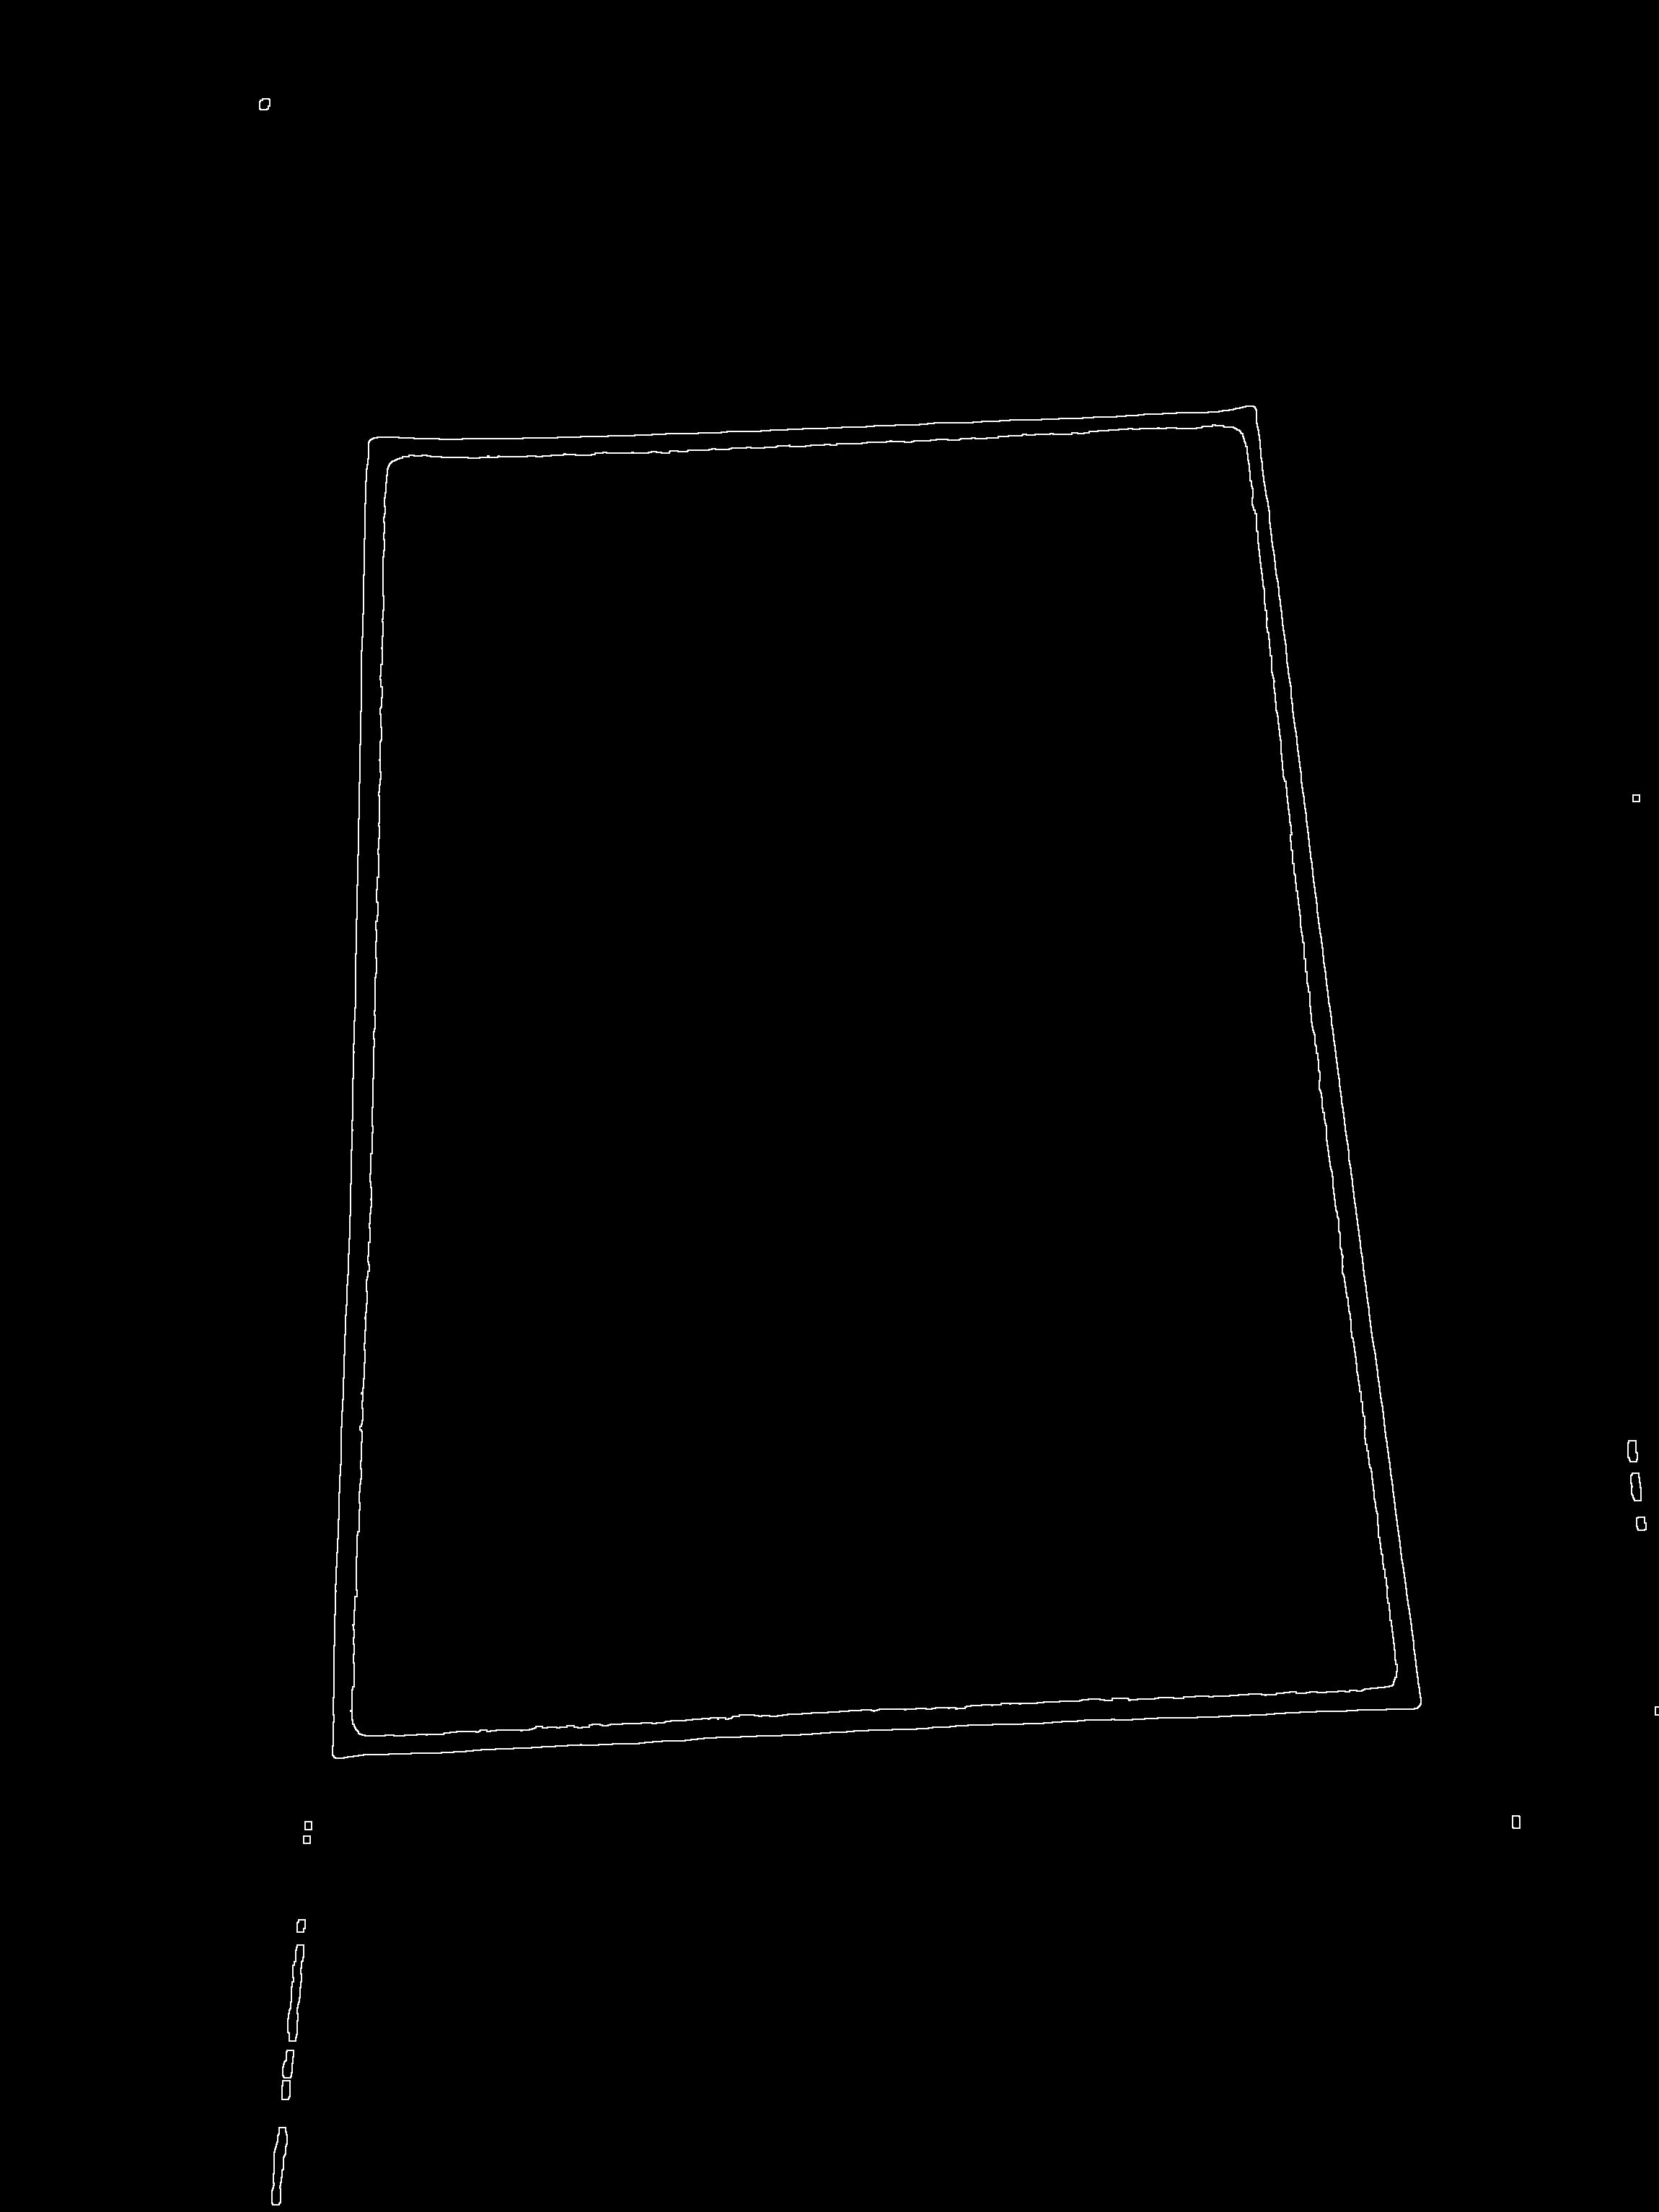
\includegraphics[width=0.37\textwidth]{./fig/desenvolvimento/thresholded_edge_sobel}
    \label{subfig:bordas-sobel}
   }
   \caption{{\subref{subfig:adp-thres}} e {\subref{subfig:bordas-sobel}} Resultado do processamento da imagem }
  \label{fig:subfiguras}
\end{figure}

Podemos notar na Figura \ref{subfig:adp-thres} que o contorno do objeto ficou bem definido agora podemos aplicar os algoritmos para detecção de bordas. Foram testados os algoritmos  Canny e Sobel, sendo o Sobel o que mostrou melhor resultado combinando os filtros horizontal e vertical como pode ser visto na figura \ref{subfig:bordas-sobel}. 

\subsection{Segmentação}
\label{sec:segmentacao}

Após a detecção das bordas com o algoritmo Sobel, foi utilizado a função \textbf{findContours} da Opencv que faz uma varredura na imagem binarizada resultante do processo do Sobel e extrai um vetor de pontos (x,y) do contorno dos objetos encontrados na imagem, os parâmetros que melhor se ajustaram para essa função foram \textbf{RETR EXTERNAL} para o modo de retorno dos contornos e \textbf{CHAIN APPROX SIMPLE} para o método de aproximação dos contornos, isso quer dizer que será retornado os contornos mais externos e com o menor número de pontos possíveis  para identificar a forma presente na imagem isso aumenta a performance do algoritmo. Como na imagem pode haver mais de um objeto ou ruídos, é realizado um cálculo da área de cada objeto e realizado uma ordenação  descendente por área, é feito um laço e validado somente as áreas maiores de 260.000,  em seguida aplico a função  \textbf{approxPolyDP } da Opencv, essa função reduz ainda mais a quantidade de pontos do contorno do objeto, tornando possível identificar o shape do objeto, no nosso caso a folha do teste que tem um formato de retângulo, isso é validado no caso da forma tiver 4 vértices então achamos nosso ROI(Region of interest). Na figura \ref{subfig:roi-img} podemos ver o resultado desse processo, o retângulo verde por cima da folha são as coordenas da ROI.


\begin{figure}[h]
 \centering
  \subfigure[][Localização da região de interesse para segmentação.]
   {
    
    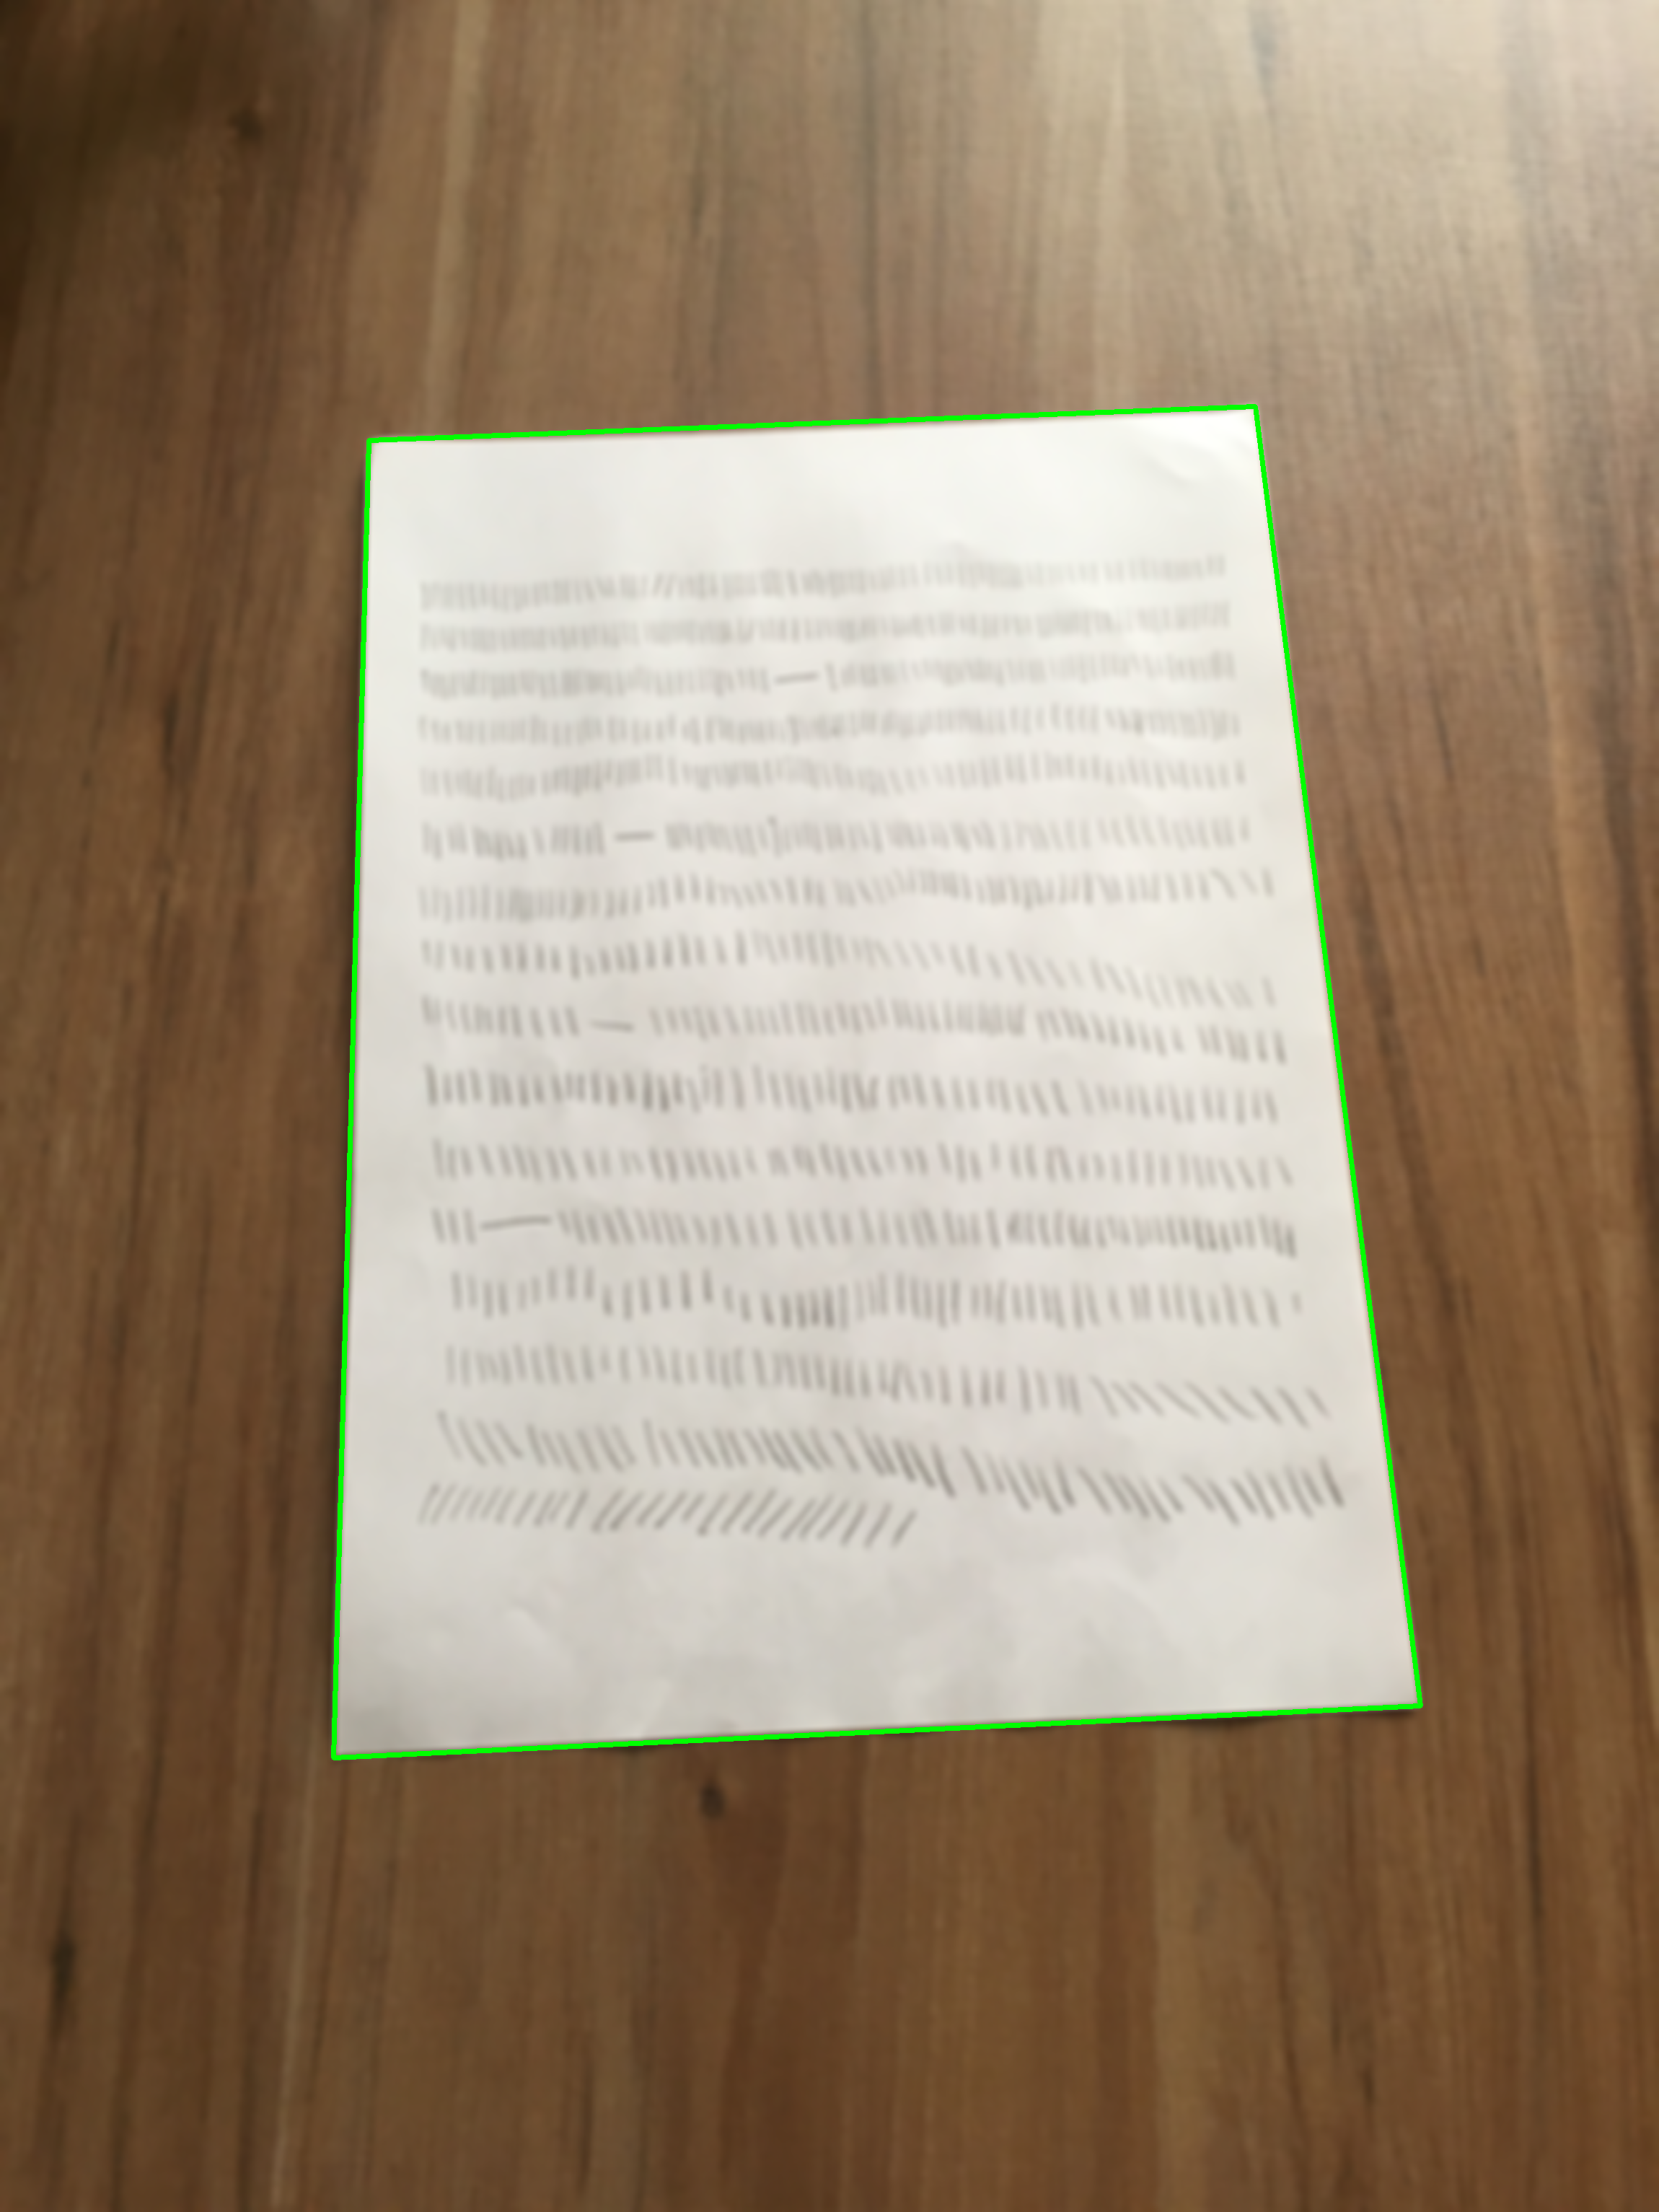
\includegraphics[width=0.37\textwidth]{./fig/desenvolvimento//flat_object_resized_roi}
    \label{subfig:roi-img}
   } \qquad
  \subfigure[Objeto de interesse segmentado.]
   {
    \includegraphics[width=0.40\textwidth]{./fig/desenvolvimento/correcao_perspectiva}
    \label{subfig:img-segmentada}
   }
   \caption{{\subref{subfig:roi-img}} e {\subref{subfig:img-segmentada}} Resultado do processamento segmentação da imagem }
  \label{subfig:segmentacao}
\end{figure}

Após a obtenção das coordenadas da nossa ROI é realizado o processo de segmentação. Nesse processo é realizado a separação entre o objeto detectado e o fundo da imagem, como já temos o vetor com as coordenas (x,y) do objeto, é feito um recorte na imagem original utilizando essas coordenadas realizando assim a segmentação. É realizado também a correção de perspetiva do objeto, utilizando a função \textbf{warpPerspective} da Opencv, isso melhora na detecção dos palos.

\section{Identificação dos palos}
\label{sec:ident-palos}

Após a segmentação da folha com o teste dos palos, são aplicados alguns algoritmos  de melhoria na imagem por histograma e operações morfológicas para que possa se identificar os palos.
\subsection{Pré-processamento}
\label{sec:pre-proce}
Nessa etapa a imagem é convertida para o espaço de cores LAB,  onde a camada L é responsável por armazenar somente os dados de luminosidade da imagem em seguida é aplicado uma correção do contraste por equalização adaptativa do histograma utilizando a função da Opencv \textbf{createCLAHE} essa abordagem é mais eficiente em imagens onde pode haver maior variação de luminosidade, pois o ajuste do contraste por histograma ocorre em pedaços da imagem e não na imagem de maneira global. Em seguida são realizadas  transformações morfológicas  com a função \textbf{morphologyEx} da Opencv foram utilizadas as operações de erosão e dilatação e a \textbf{BLACKHAT}, depois foi aplicado um filtro de suavização  para redução de ruídos, em seguida a imagem foi binarizada utilizando a função \textbf{threshold}.
Na imagem \ref{subfig:roi-seg}  temos o resultado da aplicação dessas técnicas de processamento.

\begin{figure}[h]
 \centering
  \subfigure[][Imagem após equalização adaptativa por histograma.]
   {
    
    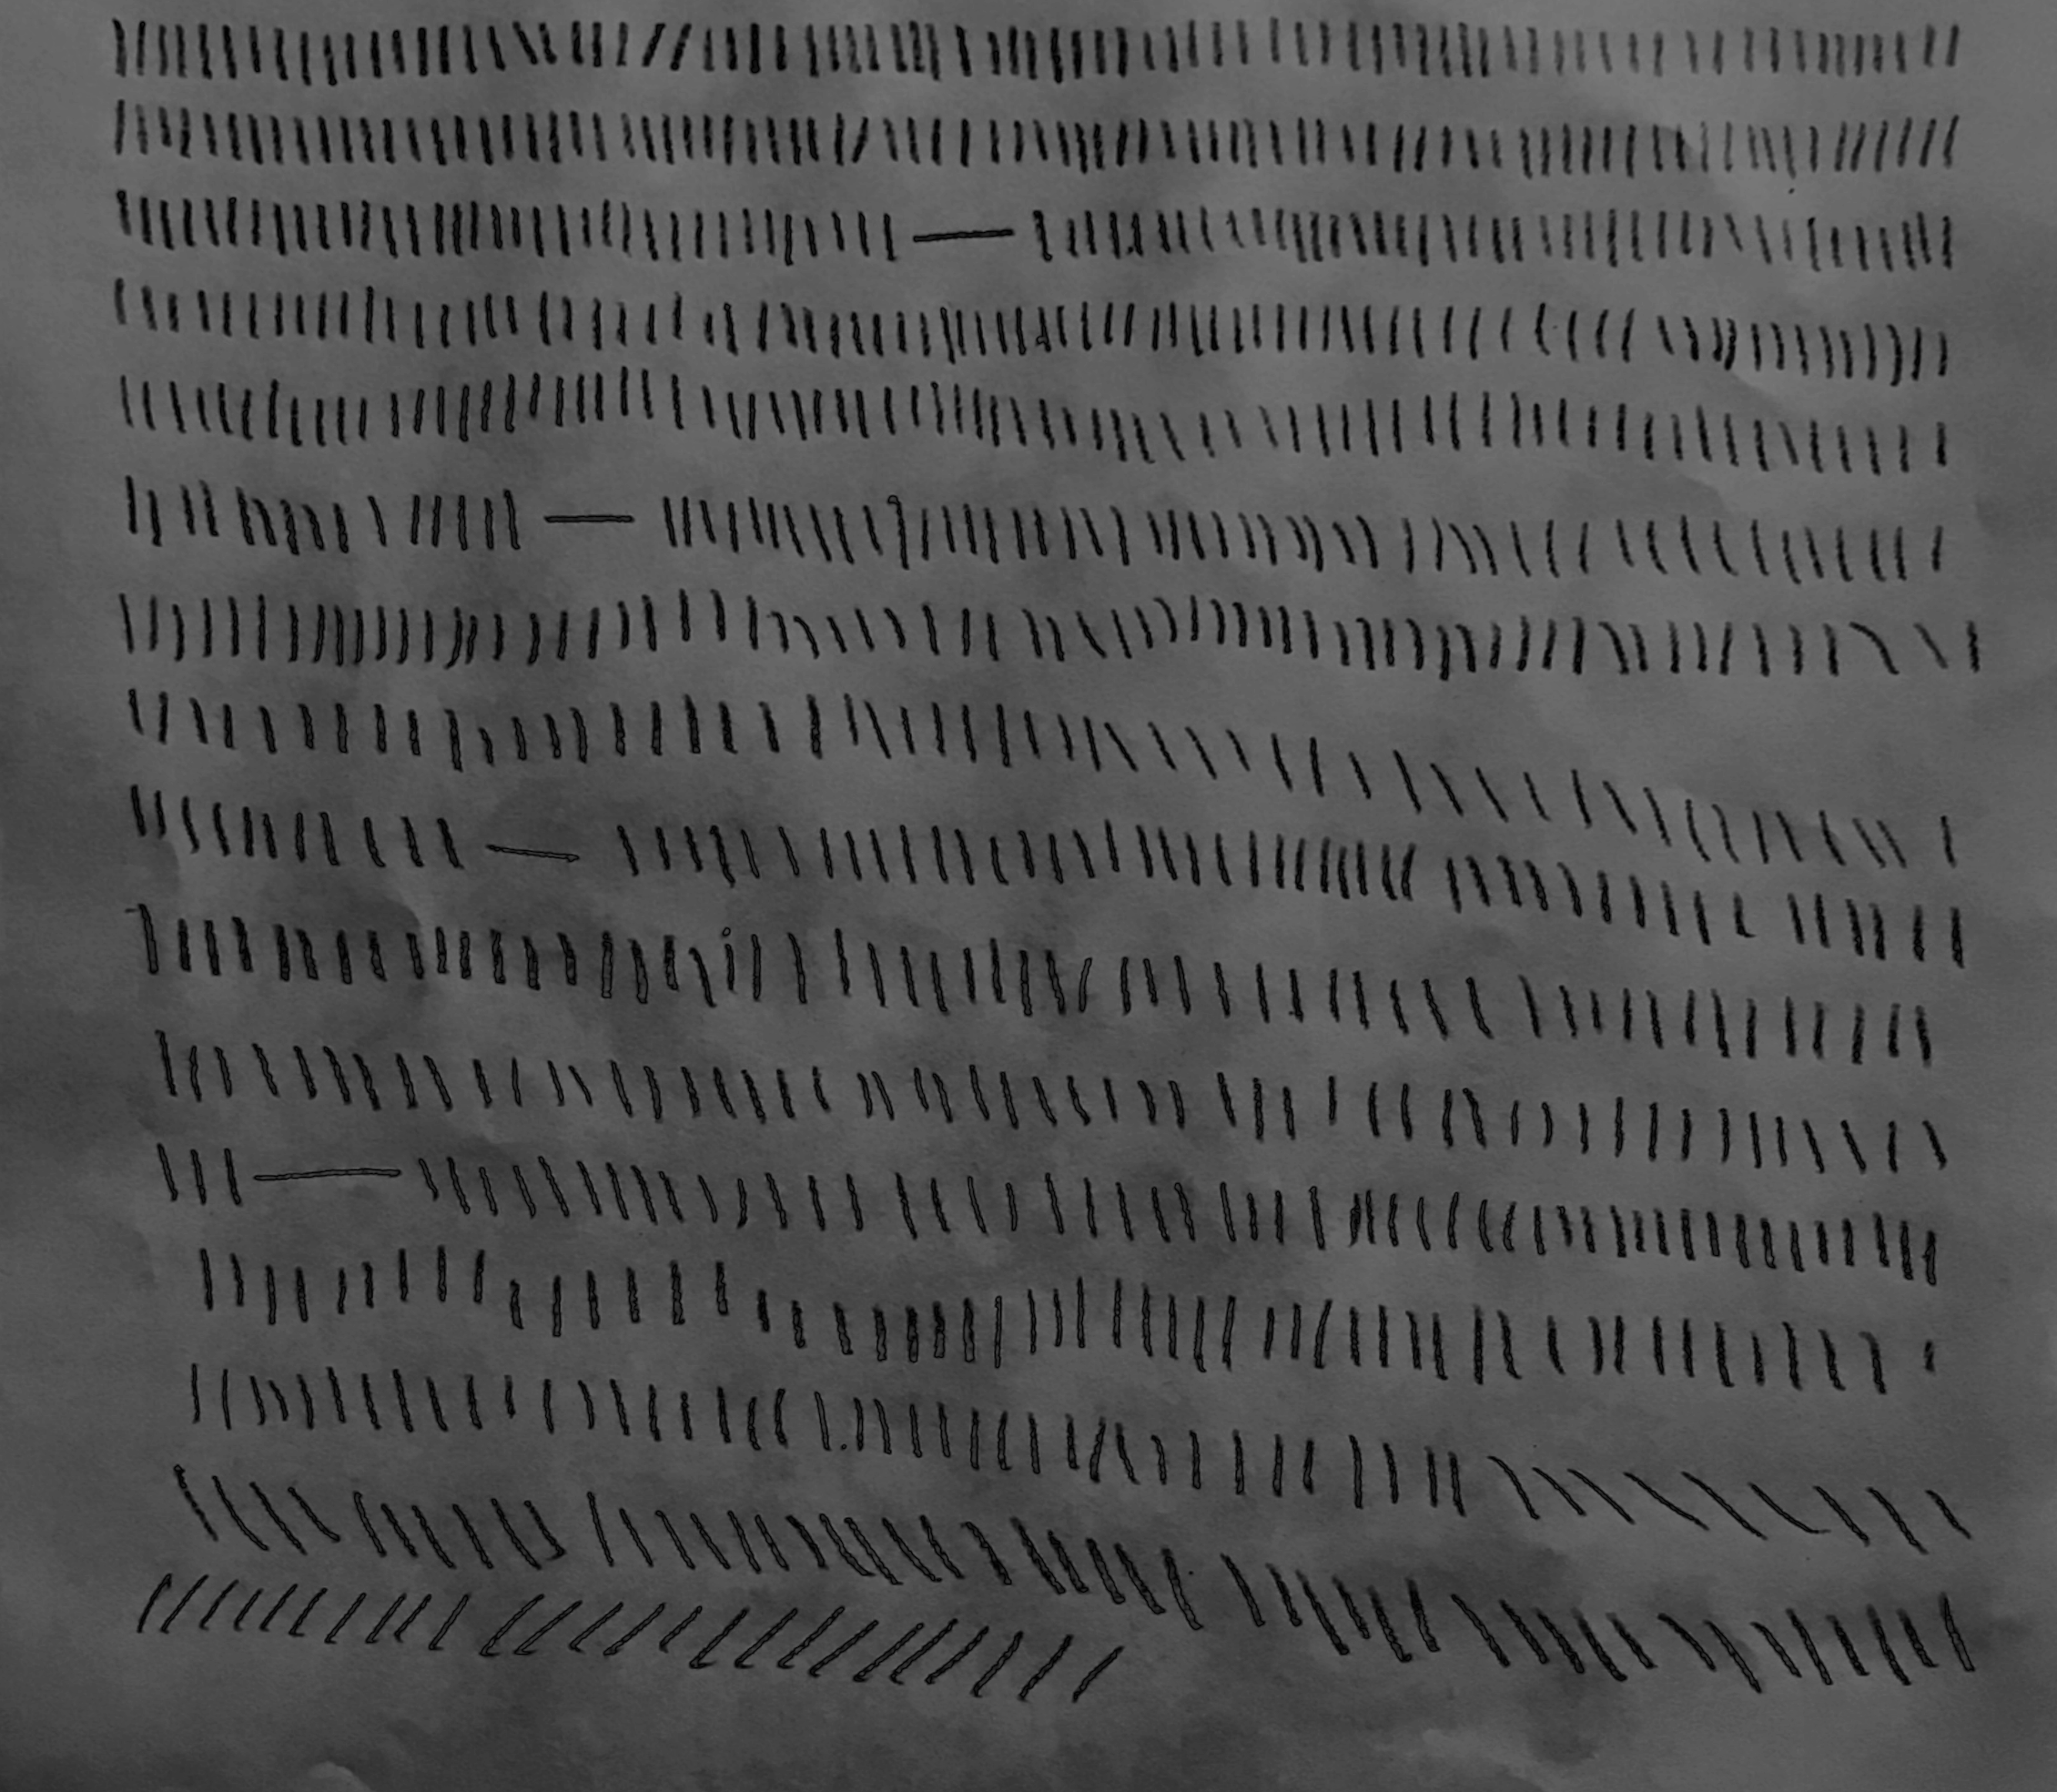
\includegraphics[width=0.32\textwidth]{./fig/desenvolvimento//img_clahe}
    \label{subfig:roi-clahe}
   } \qquad
    \subfigure[][Imagem apos aplicação a transformação morfológica BLACKHAT.]
   {
    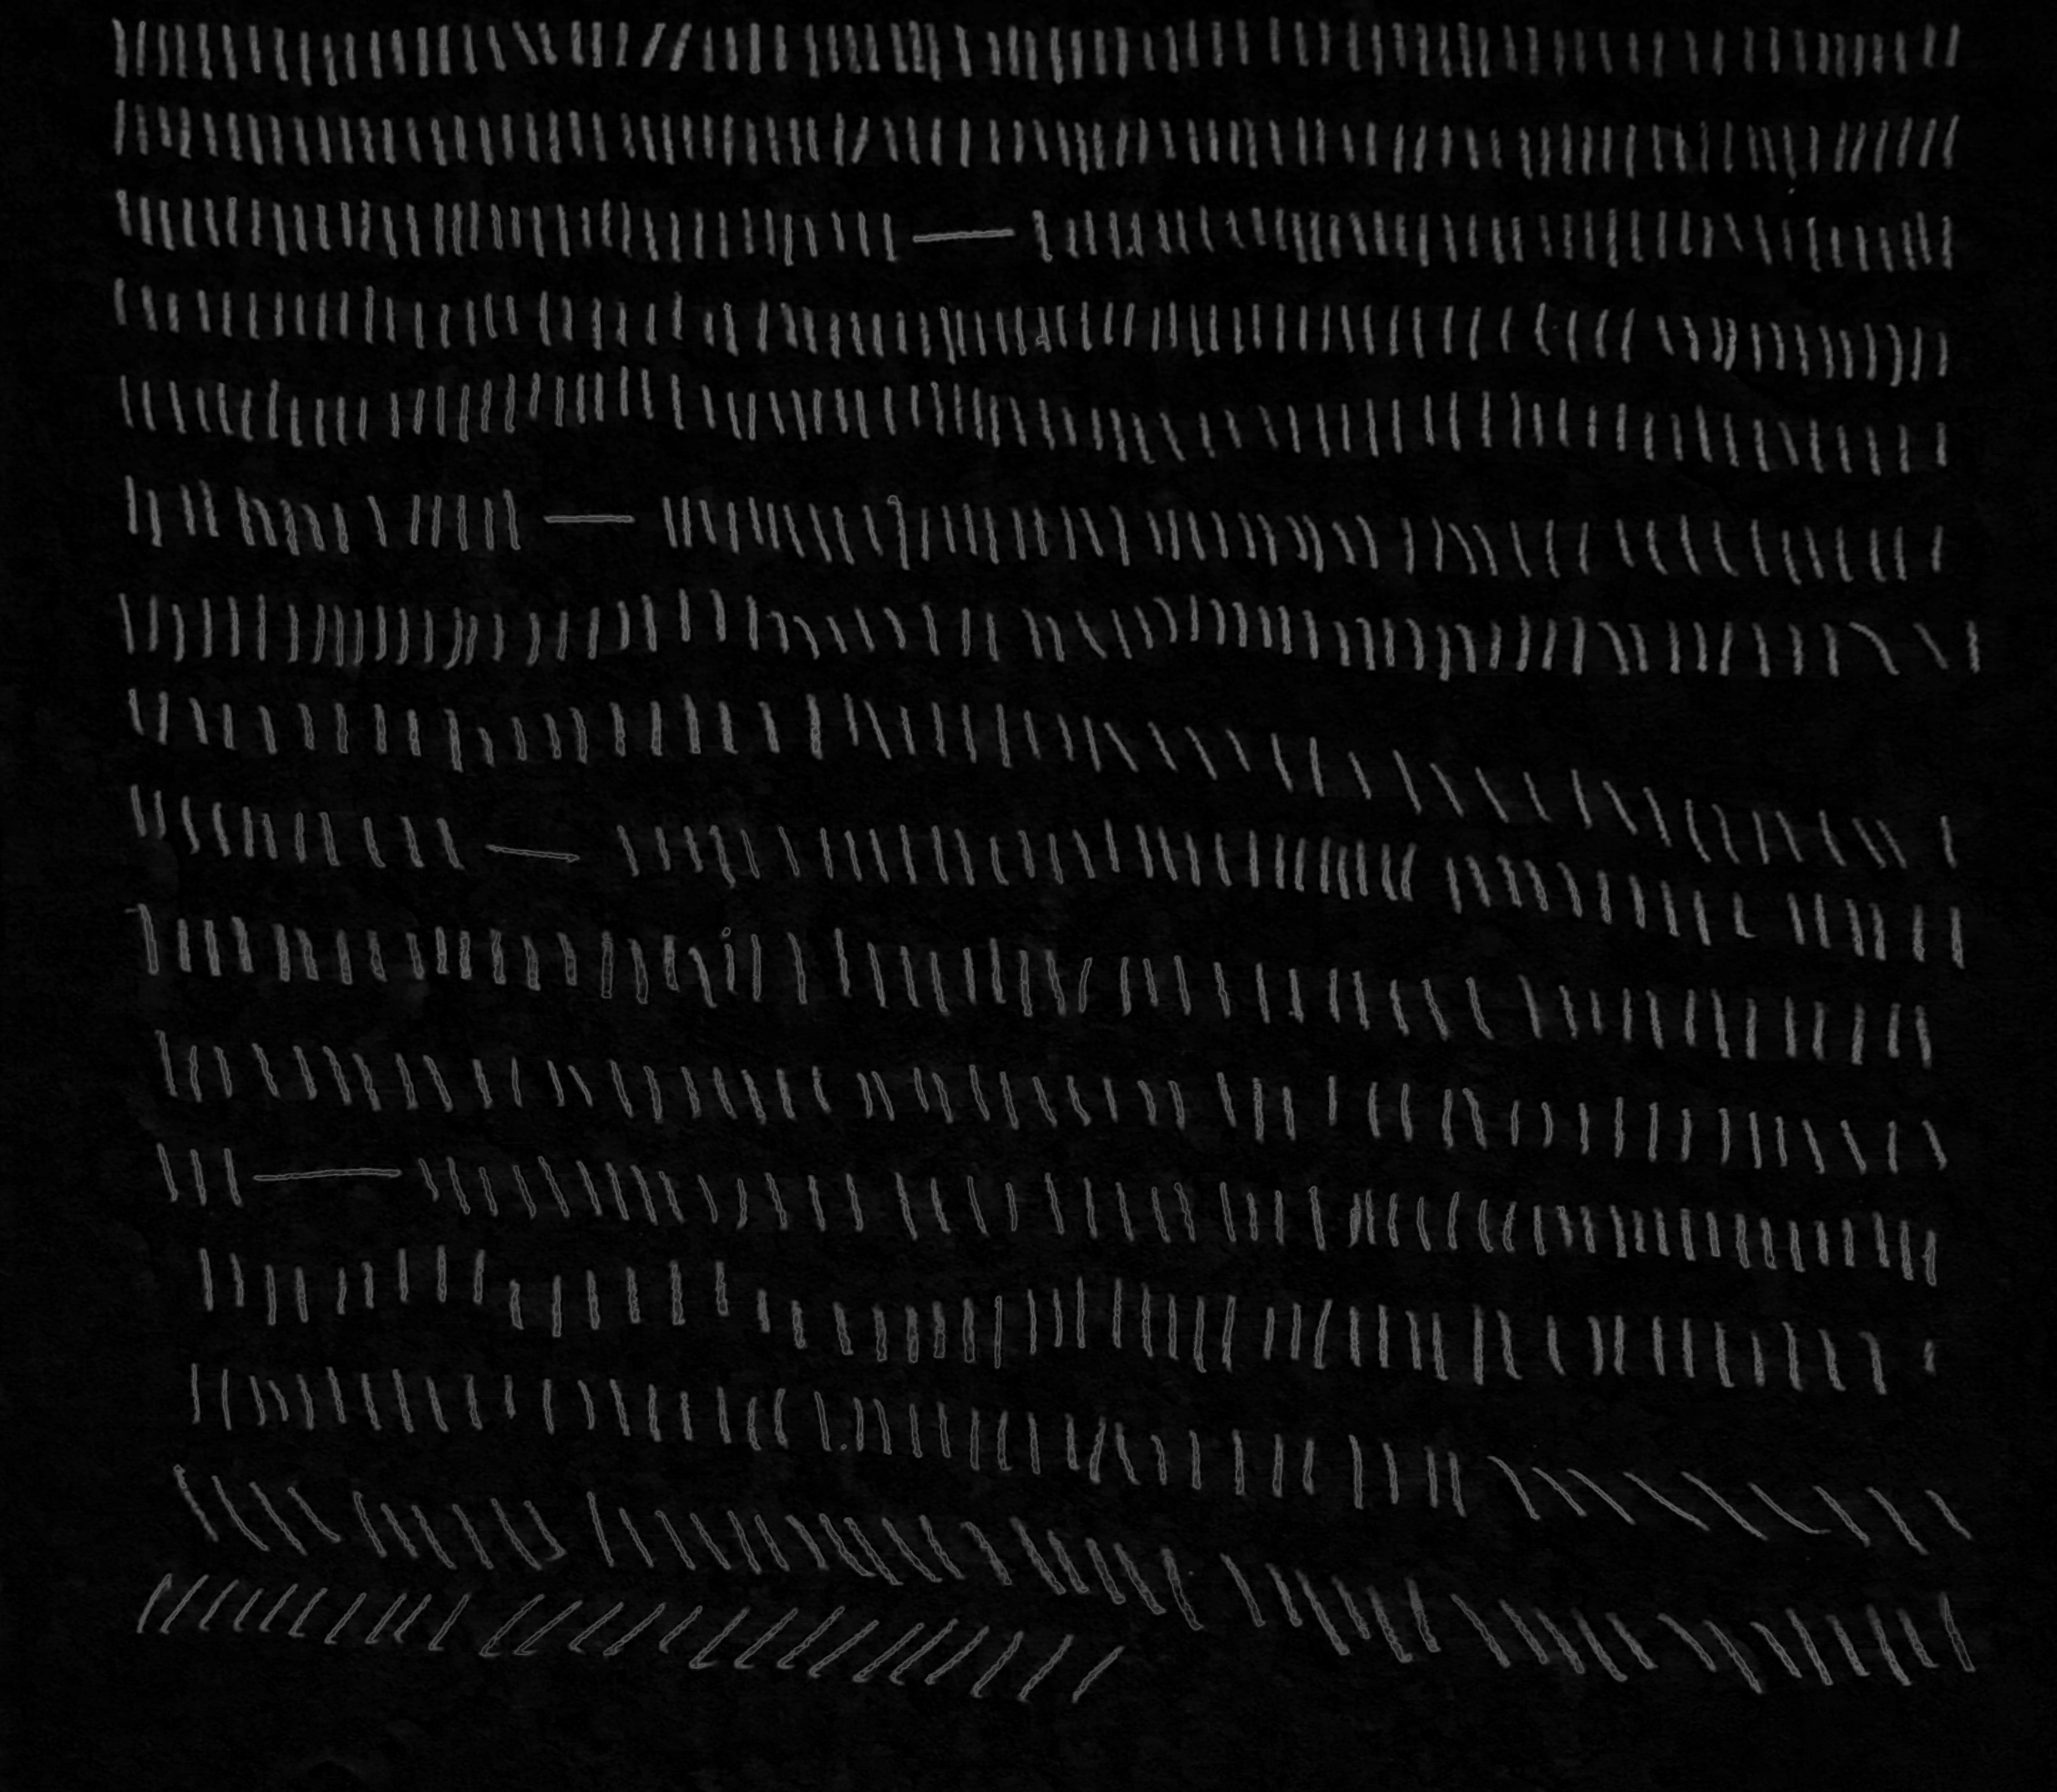
\includegraphics[width=0.32\textwidth]{./fig/desenvolvimento//blackhat}
    \label{subfig:roi-blck}
   } \qquad
  \subfigure[Imagem binarizada.]
   {
    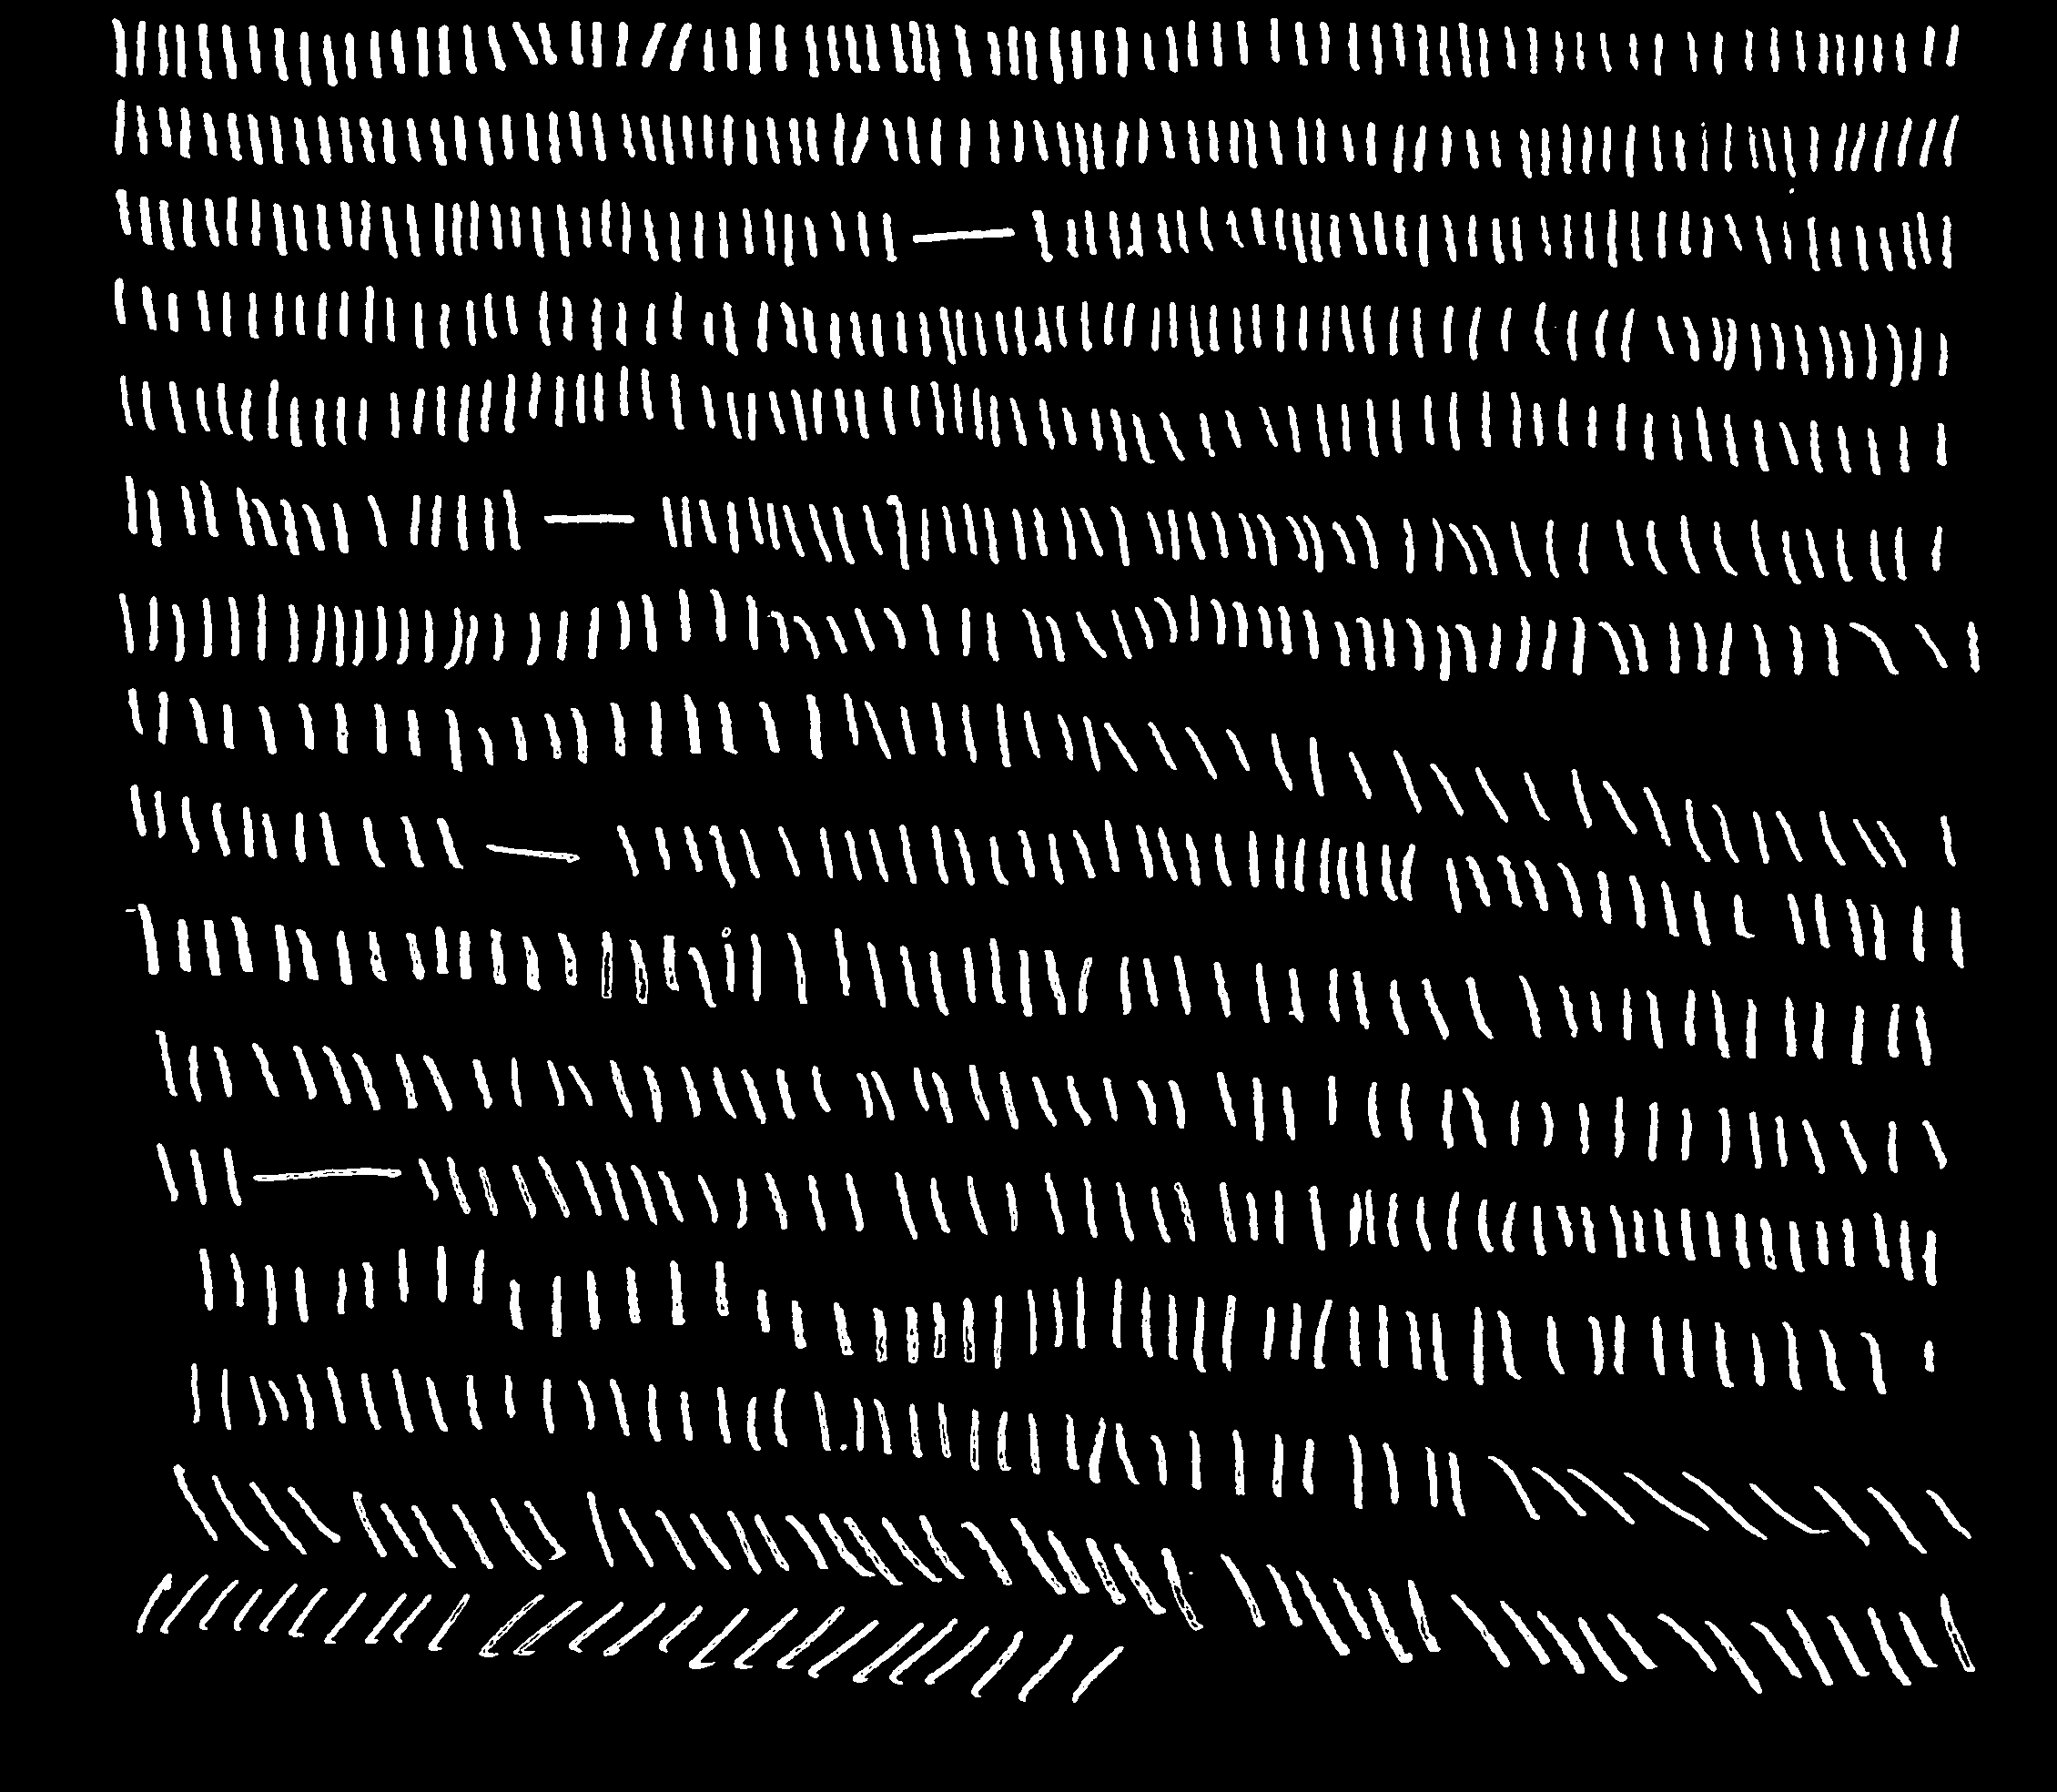
\includegraphics[width=0.32\textwidth]{./fig/desenvolvimento/binarization}
    \label{subfig:roi-bin}
   }
   \caption{{\subref{subfig:roi-clahe}} , {\subref{subfig:roi-blck}} e {\subref{subfig:roi-bin}} Resultado do processamento e binarização da imagem }
  \label{subfig:roi-seg}
\end{figure}

Após a binarização é utilizado a função \textbf{findContours} da Opencv com os parâmetros \textbf{RETR EXTERNAL}  que diz a função para retornar os contornos mais externos e o parâmetro \textbf{CHAIN APPROX SIMPLE} que utiliza menos pontos para os contornos dos objetos encontrados na imagem, assim como foi feito na parte de localização da folha do teste palográfico, essa função retorna uma lista com as coordenadas x e y de cada objeto encontrado na imagem, no caso, os palos. Porém, ainda pode haver ruído nessa lista, com o objetivo de removê-los, é feito uma validação que remove os objetos que tiverem um valor para o x muito próximo da margem da folha  e cuja área é muito pequena ou muito grande, então são removidos da lista de palos válidos.

\section{Contagem dos palos}
\label{sec:ident-palos}

O processo de contagem dos palos precisa ser linha a linha da direita para esquerda até chegar no traço horizontal, em seguida recomeça-se a contagem e repete-se esse processo para os 5 tempos do teste. Pensando nisso foi desenvolvido um algorítimo que localiza o primeiro palo e a partir dele sempre pega o palo mais próximo. Para isso é calculado a distância entre os palos utilizando as coordenadas cartesianas (x,y) de cada palo. A fórmula utilizada é a distância euclidiana. $d_{ab}=\sqrt{(x_b - x_a)^2 + (y_b - y_a)^2}$  a partir disso é feito a ordenação dos palos para que o processo de contagem fique correto.

Em seguida depois de ordenado os palos é feito a contagem  nos 5 intervalos de tempo. Com essa informação verifica-se a diferença de palos de um intervalo para o outro e somamos essa diferença para calcularmos o NOR (Nível de Oscilação Rítmica e poderíamos calcular a produtividade e fazer o gráfico de rendimento. A imagem \ref{fig:ord-contagem} tem o resultado desse processo.

\begin{figure}[H]
 \centering
 \includegraphics[width=0.70\textwidth]{./fig/desenvolvimento/final}
 \caption{Resultado da ordenação e contagem dos palos.}
 \label{fig:ord-contagem}
\end{figure}






\chapter{Resultados e Discussões}
\label{cap:resultados}

% - - - - - - - - - - - - - - - - - - - - - - - - - - - - - - - - - - -------
Neste capítulo serão apresentados os testes no protótipo e a análise dos resultados. Para execução dos testes, foram levadas em consideração algumas possíveis restrições para captura da imagem pelo celular, para que não afete o funcionamento do algoritmo. 

A folha do teste deve estar em uma superfície plana e o celular deve estar posicionado a uma distancia de aproximadamente 30 cm da folha do teste, ele deve ficar paralelo a superfície do teste para uma melhor captura da imagem, deve se respeitar também todas as restrições vistas na Seção 3.3.1. Foram utilizadas no teste as folhas do modelo II conforme seção 2.2.1. Ao todo, foram utilizadas 10 imagem do teste palográfico.

Na tabela \ref{tab:result}  temos o resultado da contagem para as imagens utilizadas nos testes. Foi feito uma comparação entre a contagem manual dos palos e a contagem feito pelo protótipo, temos também a quantidades de palos detectados pelo contador que não estão presentes no total real, temos a quantidade de palos não detectados pelo contador e o percentual de acertos pelo protótipo. Foi denominado falso positivo quando o algoritmo detecta palos a mais que a quantidade feita na contagem manual e falso negativo quando alguns palos não são detectados.
No decorrer do experimento, foi observado que esses erros de detecção ocorrem na etapa de segmentação. Os falsos positivos geralmente ocorrem quando o palo esta meio apagado ou quando o palo não tem um tonalidade de cinza constante. Gerando mais objetos que a quantidade real, como pode ser visto na Figura \ref{fig:palo-seg}.

\begin{figure}[H]
 \centering
 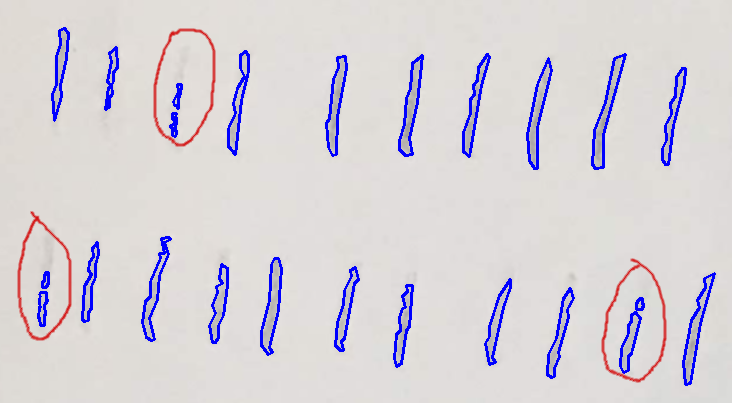
\includegraphics[width=0.50\textwidth]{./fig/resultado-analise/seg-palo}
 \caption{Segmentação de falsos positivos.}
  Fonte: O autor.
 \label{fig:palo-seg}
\end{figure}

Já os falsos negativos ocorrem quando os palos estão muito próximos ou encostado um no outro, dificultando a segmentação fazendo com que dois ou mais palos sejam contados como apenas um. Como pode ser visto na Figura \ref{fig:palo-seg}  .

\begin{figure}[H]
 \centering
 \includegraphics[width=0.50\textwidth]{./fig/resultado-analise/seg-palos}
 \caption{Segmentação de falsos negativos.}
  Fonte: O autor.
 \label{fig:palo-seg}
\end{figure}


\begin{table*}[hp]
\centering
\begin{tabular}{|l|l|l|l|l|l|}
\hline
\textbf{Teste} & \textbf{\begin{tabular}[c]{@{}l@{}}Contagem \\ Manual\end{tabular}} & \textbf{\begin{tabular}[c]{@{}l@{}}Contagem \\ prototipo\end{tabular}} & \textbf{\begin{tabular}[c]{@{}l@{}}Falso \\ positivo\end{tabular}} & \textbf{\begin{tabular}[c]{@{}l@{}}Falso \\ negativo\end{tabular}} & \textbf{\%Acerto} \\ \hlin
1              & 805    & 785       & 0      & 20    & 97,51\%        \\ \hline
2              & 620    & 620       & 0      & 0      & 100\%           \\ \hline
3              & 688    & 684       & 0      & 4      & 99,41\%        \\ \hline
4              & 632    & 633       & 1      & 0      & 99,84\%        \\ \hline
5              & 945    & 945       & 0      & 0      & 100\%           \\ \hline
6              & 577    & 575       & 0      & 2      & 99,65\%        \\ \hline
7              & 856    & 858       & 3      & 1      & 99,53\%        \\ \hline
8              & 818    & 815       & 0      & 3      & 99,75\%        \\ \hline
9              & 907    & 900       & 0      & 7      & 99,22\%        \\ \hline
10            & 1008  & 995       & 0      & 13    & 98,71\%        \\ \hline

\end{tabular}
\caption{Comparação dos resultados da contagem manual com a contagem feito pelo protótipo}
\label{tab:result}
\end{table*}

Somando-se os palos de todos os testes temos 7856 palos, com apenas  54 erros cometidos pelo protótipo, obtendo uma taxa de acerto no geral de 99.31\% o que é um resultado promissor. Podemos notar que a diferença entre os valores reais e os obtidos na contagem é pequena sendo a maior no teste número 1 com 20 erros. Os melhores resultados foram nos testes numero 2 e 5 contabilizando a quantidade exata dos palos. Nas demais, a menor taxa de acerto foi no teste numero 1, com valor de 97,51\%  de acerto.

O protótipo resultante deste trabalho  mostrou-se promissor, mostrando que o uso de técnicas de processamento de imagens e visão computacional tem se tornando de grande ajuda na resolução de problemas do dia a dia, como podemos ver nos trabalho de \cite{SILVA2012},  que utiliza as mesmas técnicas utilizadas neste trabalho e que também mostra resultados positivos. Ainda que os resultados tenham sido positivos,  é imprescindível que seja realizado mais testes de maneira exaustiva para um melhor grau de acurácia e confiabilidade, porém para o propósito deste trabalho os resultados são satisfatórios.

Uma característica importante neste protótipo é que ele utiliza de imagens obtidas por celular, não há a necessidade de aquirir nenhum equipamento específico para a contagem dos palos, como acontece no \textit{software} \cite{skip2018}.








 \chapter{Conclusão}
\label{cap:conclu}
% - - - - - - - - - - - - - - - - - - - - - - - - - - - - - - - - - - -

O desenvolvimento deste trabalho acerca da utilização de técnicas de Processamento de Imagens e Visão Computacional para um protótipo de contagem dos palos em um teste palográfico proporcionou um aprendizado razoável sobre o tema.  Com conclusão deste estudo podemos responder a questão levantada no Capitulo 1, pode ser verificado que se respeitado algumas restrições conforme Seção 3.3.1 é possível a criação de um protótipo para a contagem dos palos a partir de imagens de celular.

O trabalho resultante é baseado em técnicas de processamento digital de imagens e visão computacional, que são áreas crescentes na computação, devido a sua capacidade de abranger inúmeros segmentos de aplicações. Outra particularidade foi a utilização da biblioteca OpenCV, a mesma demonstrou-se muito eficiente e de simples utilização reverberando no bom resultado.

Os resultados dos testes mostram um grande potencial do protótipo, pois se mostrou eficaz, devido a sua baixa taxa de erro, o que justifica sua utilização em alternativa à contagem manual.  Além de uma maior precisão na contatem é possível obter o resultado mais rapidamente, o que possibilita um ganha de tempo na rotina do profissional aplicador do teste palográfico.

Como possíveis trabalhos futuros, pode-se ressaltar:
Ainda que o protótipo tenha se mostrado eficaz, ainda precisa de alguns ajustes a serem realizados de modo a aperfeiçoar os resultados e torná-lo mais robusto às falhas.

Na etapa de segmentação poderia ser utilizado outros parâmetros de limiarização de modo a melhorar a identificação e separação dos palos. Melhorar, por exemplo, a sensibilidade à variação de luminosidade.

Desenvolver o aplicativo \textit{mobile} para utilizar em tempo real o algoritmo de contagem dos palos, mostrando gráficos da análise quantitativa do teste palográfico.

Desenvolver um algoritmo de visão computacional para análise qualitativa do teste palográfico utilizando técnicas de inteligência artificial como Redes Neurais, para classificação dos palos com maior precisão.

A implementação dessas e outras melhorias fazem parte dos trabalhos a serem realizados no futuro.









% \chapter{Elementos do texto}
\label{cap:texto}

% - - - - - - - - - - - - - - - - - - - - - - - - - - - - - - - - - - -
\section{Figuras}
\label{sec:figs} 
Rótulos de figuras e tabelas devem ser centralizados se tiverem até uma linha (Figura~\ref{fig:exemploFig1}), caso contrário devem estar justificados e identados em ambas as margens, como mostrado na Figura ~\ref{fig:exemploFig2}. Essa formatação já é realizada automaticamente pela classe \textsf{inf-ufg}.

Os compiladores \LaTeX\ provêem um mecanismo bastante simples para inclusão de figuras, o que pode ser feito com o auxílio de várias classes auxiliares (as mais comuns são \verb|graphic| e \verb|graphicx|). A classe \verb|inf-ufg| usa o comando \verb|\includegraphics|, da classe \verb|graphicx|, para a inclusão de figuras e não é necessário você colocar a extensão do arquivo neste comando. Por exemplo, para a figura \ref{fig:exemploFig1} os comandos usados foram:
\begin{Verbatim}
 \begin{figure}[htb]
  \centering
  \includegraphics[width=0.40\textwidth]{./fig/exemploFig1}
  \caption{Uma figura típica.}
  \label{fig:exemploFig1}
 \end{figure}
\end{Verbatim}

Ao se usar o compilador \LaTeX, as figuras podem estar nos formatos \textit{eps} e \textit{ps}. Ao se usar o PDF\LaTeX, as figuras podem estar nos formatos \textit{png}, \textit{jpg}, \textit{pdf} e \textit{mps}. A classe \verb|graphicx| também pode ser usada para a inclusão de figuras, nos formatos listados, ao se usar o PDF\LaTeX. Os comandos necessários são os mesmos ao se incluir figuras ao se usar o compilador \LaTeX. O uso do comando \verb|\includegraphics| faz com com que PDF\LaTeX\ procure primeiro por figuras com extensão \textit{pdf}, depois \textit{jpg}, depois \textit{mps} e por último \textit{png}. Aqui também não é necessário especificar a extensão do arquivo.

Para a inclusão das figuras \ref{fig:exemploFig1} à \ref{fig:exemploFig3} os comandos usados, tanto no \LaTeX\ quanto no PDF\LaTeX, seriam os mesmos. É claro que em cada caso devem estar disponíveis as figuras nos formatos suportados por cada compilador. Por exemplo, para a inclusão da figura \ref{fig:exemploFig3} foram usados:
\begin{Verbatim}
 \begin{figure}[H]
  \centering
  \includegraphics[width=0.40\textwidth]{./fig/exemploFig3}
  \caption{Figura incluída no texto com a classe graphicx.}
  \label{fig:exemploFig3}
\end{figure}
\end{Verbatim}

\begin{figure}[H]
 \centering
  \includegraphics[width=0.40\textwidth]{./fig/exemploFig1}
 \caption{Uma figura típica.}
 \label{fig:exemploFig1}
\end{figure}

\begin{figure}[H]
 \centering
 \includegraphics[width=0.30\textwidth]{./fig/exemploFig2}
 \caption{Esta figura é um exemplo de um rótulo de figura que ocupa mais de uma linha, devendo ser identado e justificado.}
 \label{fig:exemploFig2}
\end{figure}

\begin{figure}[H]
 \centering
  \includegraphics[width=0.40\textwidth]{./fig/exemploFig3}
  \caption{Figura incluída no texto com a classe graphicx.}
 \label{fig:exemploFig3}
\end{figure}

\subsection{Subfiguras}
\label{subsec:subfigs} 
A classe \verb|subfigure| pode ser usada para a inclusão de figuras dentro de figuras (consulte a documentação da classe para maiores detalhes). Por exemplo, a Figura \ref{fig:subfiguras} contém duas subfiguras. Estas podem ser referencidas por rótulos independentes, ou seja, podem ser referenciadas como Figuras \ref{subfig:ex1} e \ref{subfig:ex2} ou Subfiguras \subref{subfig:ex1} e \subref{subfig:ex2}.
\begin{figure}[h]
 \centering
%   \subfigure[][Primeira subfigura.]
  \subfigure[][Primeira subfigura.]
   {
    \includegraphics[width=0.35\textwidth]{./fig/exemploFig1}
    \label{subfig:ex1}
   } \qquad
  \subfigure[Segunda subfigura (um pedaço).]
   {
    \includegraphics[width=0.30\textwidth]{./fig/exemploFig2}
    \label{subfig:ex2}
   }
   \caption{{\subref{subfig:ex1}} e {\subref{subfig:ex2}} representam dois exemplos do uso de subfiguras dentro de uma única figura.}
  \label{fig:subfiguras}
\end{figure}

A figura \ref{fig:subfiguras} foi incluída com os comandos listados a seguir. Observe que há rótulos independentes para cada uma das subfiguras e um rótulo geral para a figura, os quais podem ser todos referenciados.
\begin{Verbatim}
\begin{figure}[h]
 \centering
  \subfigure[Primeira subfigura.]
   {
    \includegraphics[width=0.35\textwidth]{./fig/exemploFig1}
    \label{subfig:ex1}
   } \qquad
  \subfigure[Segunda subfigura (um pedaço).]
   {
    \includegraphics[width=0.30\textwidth]{./fig/exemploFig2}
    \label{subfig:ex2}
   }
   \caption{{\subref{subfig:ex1}} e {\subref{subfig:ex2}} representam
             dois exemplos do uso de subfiguras dentro de uma única
             figura.}
  \label{fig:subfiguras}
\end{figure}
\end{Verbatim}
 Caso uma subfiguras não tenha rótulo, para evitar que o apenas o número da mesma apareça na Lista de Figuras, use o comando \verb|\subfigure[][]|.  Caso uma subfigura tenha rótulo e deseja-se evitar que a mesma apareça na Lista de Figuras, use o comando \verb|\subfigure[][Rótulo]|.
%% - - - - - - - - - - - - - - - - - - - - - - - - - - - - - - - - - - -
\section{Tabelas}
\label{sec:tabs} 
Em tabelas, deve-se evitar usar cor de fundo diferente do branco e o uso de linhas grossas ou duplas. Ao relatar dados empíricos, não se deve usar mais dígitos decimais do aqueles que possam ser garantidos pela sua precisão e reprodutibilidade. Rótulos de tabelas devem ser colocados
antes das mesmas (veja a Tabela \ref{tab:MarcMNem}).

\begin{table*}[hp]
\centering
\caption{Conteúdo do diretório \cite{Mar2004} }
\label{tab:MarcMNem} 
\begin{tabular}{|c|c|c|c|c|c|c|}
\hline Tag & Comprimento & Início &   & Tag & Comprimento & Início \\ 
\hline 001 & 0020 & 00000 && 100 & 0032 & 00235\\ 
\hline 003  0004 & 00020 && 245 & 0087 & 00267\\ 
\hline 005 & 0017 & 00024 && 246 & 0036 & 00354\\ 
\hline 008 & 0041 & 00041 && 250 & 0012 & 00390\\ 
\hline 010 & 0024 & 00082 && 260 & 0037 & 00402\\ 
\hline 020 & 0025 & 00106 && 300 & 0029 & 00439\\ 
\hline 020 & 0044 & 00131 && 500 & 0042 & 00468\\ 
\hline 040 & 0018 & 00175 && 520 & 0220 & 00510\\ 
\hline 050 & 0024 & 00193 && 650 & 0033 & 00730\\ 
\hline 082 & 0018 & 00217 && 650 & 0012 & 00763\\ 
\hline 
\end{tabular} 
\end{table*}

%% - - - - - - - - - - - - - - - - - - - - - - - - - - - - - - - - - - -
\section{Algoritmos}
\label{sec:algor} 
Algoritmos devem ser representados no formato do Algoritmo \ref{alg:poten}, que foi descrito com o uso da classe \textsf{algorithm2e}. A rigor não é obrigatório o uso dessa classe, contudo o uso da mesma permite que seja gerada automaticamente uma lista de algoritmos logo após o sumário.

\medskip
\begin{center}
\begin{minipage}{0.92\textwidth}
\begin{algorithm2e}[H]
 \DontPrintSemicolon
 \LinesNumbered
 \SetAlgoLined
 \BlankLine
 \Entrada{vetor $A[i\,.\,.\,j]$, inteiros não negativos $i$ e $j$.}
 \Saida{vetor $A[i\,.\,.\,j]$ ordenado.}
 \BlankLine
 $n \leftarrow j - i$.\;
 \eSe{$(n<4)$}
   {Ordene com $\leq 3$ comparações.}
   {Divida $A$ em $\lceil\sqrt{n}\,\,\rceil$ subvetores de comprimento máximo $\lfloor\sqrt{n}\,\rfloor$.\;
    Aplique $MSR$ a cada um dos subvetores.\;
    Intercale os subvetores.\;}
\caption{$MSR(A,i,j)$ \label {alg:poten}}
\end{algorithm2e}
\end{minipage}
\end{center}

%% - - - - - - - - - - - - - - - - - - - - - - - - - - - - - - - - - - -
\section{Códigos de Programa}
\label{sec:progs} 
Códigos de programa podem ser importados, mantendo-se a formatação original, conforme se pode ver no exemplo do Código \ref{code:prog1}. Este exemplo usa o ambiente \textsf{codigo}, definido na classe \textsf{inf-ufg}, que permite que uma lista de programas seja gerada automaticamente logo após o sumário.
\begin{center}
 \begin{minipage}{0.7\textwidth}
  \begin{codigo}[H]
   \small
   \VerbatimInput[xleftmargin=10mm,numbers=left,obeytabs=true]{./prog/insertionsort.c}
   \caption{\texttt{insertionsort()} }
   \label{code:prog1}
  \end{codigo}
 \end{minipage}
\end{center}

%% - - - - - - - - - - - - - - - - - - - - - - - - - - - - - - - - - - -
\section{Teoremas, Corolários e Demonstrações}
\label{sec:teor}
 O uso do ambiente \textsf{theorem} permite a escrita de teoremas, como no exemplo a seguir:
\begin{verbatim}
\begin{theorem}[Pitágoras]
Em todo triângulo retângulo o quadrado do comprimento
da hipotenusa é igual a soma dos quadrados dos
comprimentos dos catetos.
\end{theorem}
\end{verbatim}

O resultado é o mostrado a seguir:

\begin{theorem}[Pitágoras]
Em todo triângulo retângulo o quadrado do comprimento da hipotenusa é igual a soma dos quadrados dos comprimentos dos catetos.
\end{theorem}

Da mesma forma pode-se usar o ambiente \textsf{proof} para demonstrações de teoremas:
\begin{verbatim}
\begin{proof}
Para demonstrar o Teorema de Pitágoras \dots
\end{proof}
\end{verbatim}

Neste caso, o resultado é:
\begin{proof}
Para demonstrar o Teorema de Pitágoras \dots
\end{proof}

Além desses dois ambientes, estão definidos os ambientes \textsf{definition} (Definição), \textsf{corollary} (Corolário), \textsf{lemma} (Lema)), \textsf{proposition} (Proposição), \textsf{comment} (Observação).

%% - - - - - - - - - - - - - - - - - - - - - - - - - - - - - - - - - - -
\section{Citações Longas}
\label{sec:citacoes}

Segundo as normas da ABNT, uma citação longa (mais de 3 linhas) deve seguir uma formação especial. Para tanto foi criado o ambiente \verb|citacao|, o qual é baseado no ambiente de mesmo nome definido pelo grupo ABNTex \cite{abnt-classe-doc}:
\begin{citacao}
Uma citação longa (mais de 3 linhas) deve vir em parágrafo separado,
com recuo de 4cm da margem esquerda, em fonte menor, sem as aspas
\cite[4.4]{NBR10520:2001} e com espaçamento simples \cite[5.3]{NBR14724:2001}.
Uma regra de como fazer citações em geral não é simples. É prudente
ler \cite{NBR10520:2001} se você optar for fazer uso freqüente de citações.
Para satisfazer às exigências tipográficas que a norma pede para
citações longas, use o ambiente citacao.
\end{citacao}

Este exemplo de citação longa foi produzido com o uso do ambiente \verb|citacao|, como descrito logo a seguir:

\begin{verbatim}
\begin{citacao}
Uma citação longa (mais de 3 linhas) deve vir em parágrafo
separado, com recuo de 4cm da margem esquerda, em fonte menor,
sem as aspas \cite[4.4]{NBR10520:2001} e com espaçamento
simples \cite[5.3]{NBR14724:2001}. Uma regra de como fazer
citações em geral não é simples. É prudente ler
\cite{NBR10520:2001} se você optar for fazer uso freqüente
de citações. Para satisfazer às exigências tipográficas que a
norma pede para citações longas, use o ambiente citacao.
\end{citacao}
\end{verbatim}

%% - - - - - - - - - - - - - - - - - - - - - - - - - - - - - - - - - - -
\section{Referências Bibliográficas}
\label{sec:refs} 
Esta seção mostra exemplos de uso de referências bibliográficas com \BibTeX{} e
do comando \verb|\cite|.  Muitas das entradas listadas na página~\pageref{ref-bib}
foram obtidas de: \href{http://liinwww.ira.uka.de/bibliography/index.html}{http://liinwww.ira.uka.de/bibliography/index.html}.  Outro grande repositório de referências já em formato \BibTeX{} está disponível em:
\href{http://www.math.utah.edu/~beebe/bibliographies.html}{http://www.math.utah.edu/~beebe/bibliographies.html}.

As referências bibliográficas devem ser não ambíguas e uniformes. Recomenda-se usar números entre colchetes, como por exemplo \cite{SmiJon1999}, \cite{Knu1989} e \cite{LeeSwi2002}.
O comando \verb|\nocite| não produz texto, mas permite que a entrada
seja incluída nas referências. Por exemplo, o comando \verb|\nocite{Ber1970}| gera na lista de referências bibliográficas a entrada referente à chave \textsf{Ber1970}, mas não inclui nenhuma referência no texto. O comando \verb|\nocite{*}| faz com que todas as entradas do arquivo de dados do \BibTeX{} sejam incluídas nas referências. \nocite{Ber1970}

Existem vários livros sobre \LaTeX{}, como \cite{Bue1990,Hah1991,KopDal1995}, embora os mais famosos sejam sem dúvida \cite{Lam1996} e \cite{GooMitSam1994}. Para converter documentos \LaTeX{} para HTML veja \cite[pg.1--10]{Dra1994}.





%------------------------------------------------------------ BIBLIOGRAFIA %
\cleardoublepage
%\nocite{*} %%% Retire esta linha para gerar a bibliografia com apenas as
           %%% referências usadas no seu texto!
\arial

\bibliography{./bib/tese} %%% Nomes dos seus arquivos .bib
\label{ref-bib}

%--------------------------------------------------------------- APÊNDICES %
\apendices

%\chapter{Exemplo de um Apêndice}
\label{apend:1}
$ \alpha, \beta, \ldots, \omega $ \newline
Apêndicess são iniciados com o comando \verb|\apendices|.
Apêndicess são iniciados com o comando \verb|\apendices|.
Apêndicess são iniciados com o comando \verb|\apendices|.
Apêndicess são iniciados com o comando \verb|\apendices|.
Apêndicess são iniciados com o comando \verb|\apendices|.
Apêndicess são iniciados com o comando \verb|\apendices|.
Apêndicess são iniciados com o comando \verb|\apendices|.
Apêndicess são iniciados com o comando \verb|\apendices|.
Apêndicess são iniciados com o comando \verb|\apendices|.
Apêndicess são iniciados com o comando \verb|\apendices|.
Apêndicess são iniciados com o comando \verb|\apendices|.
Apêndicess são iniciados com o comando \verb|\apendices|.
Apêndicess são iniciados com o comando \verb|\apendices|.
Apêndicess são iniciados com o comando \verb|\apendices|.
Apêndicess são iniciados com o comando \verb|\apendices|.
Apêndicess são iniciados com o comando \verb|\apendices|.

Apêndicess são iniciados com o comando \verb|\apendices|.
Apêndicess são iniciados com o comando \verb|\apendices|.
Apêndicess são iniciados com o comando \verb|\apendices|.
Apêndicess são iniciados com o comando \verb|\apendices|.
Apêndicess são iniciados com o comando \verb|\apendices|.
Apêndicess são iniciados com o comando \verb|\apendices|.
Apêndicess são iniciados com o comando \verb|\apendices|.
Apêndicess são iniciados com o comando \verb|\apendices|.
Apêndicess são iniciados com o comando \verb|\apendices|.
Apêndicess são iniciados com o comando \verb|\apendices|.
Apêndicess são iniciados com o comando \verb|\apendices|.
Apêndicess são iniciados com o comando \verb|\apendices|.



%\input{./pos/apend_II}

\end{document}

%------------------------------------------------------------------------- %
%        F I M   D O  A R Q U I V O :  m o d e l o - t e s e . t e x       %
%------------------------------------------------------------------------- %
